\documentclass[a4paper,colorlinks=true,linkcolor=blue,urlcolor=blue,citecolor=green,bookmarks=true]{article}

% 基础宏包
\usepackage{ctex}              % 中文支持
\usepackage{graphicx}          % 图片支持
\usepackage{amsmath}           % 数学公式
\usepackage{amssymb}          % 数学符号
\usepackage{geometry}          % 页面设置
\usepackage{fancyhdr}          % 页眉页脚
\usepackage{lastpage}          % 获取总页数
\usepackage{zhnumber}          % 中文数字
\usepackage{float}             % 浮动体设置
\usepackage{subcaption}        % 支持子图

% 页面设置
\geometry{a4paper,top=2.5cm,bottom=2.5cm,left=2.5cm,right=2.5cm}

% 浮动体设置
\renewcommand{\textfraction}{0.05}
\renewcommand{\topfraction}{0.95}
\renewcommand{\bottomfraction}{0.95}
\renewcommand{\floatpagefraction}{0.35}
\setcounter{topnumber}{5}
\setcounter{bottomnumber}{5}
\setcounter{totalnumber}{10}

% 引入样式文件
% 基础包引用
\usepackage{amsmath}
\usepackage{graphicx}
\usepackage{float}
\usepackage{setspace}
\usepackage{xargs}
\usepackage{nameref}
\usepackage{appendix}
\usepackage{cite}
\usepackage{hyperref}
\usepackage{fancyref}
\usepackage{scrextend}

% 颜色定义
\usepackage[dvipsnames]{xcolor}
\definecolor{cleanOrange}{HTML}{D14D00}
\definecolor{cleanYellow}{HTML}{FFFF99}
\definecolor{cleanBlue}{HTML}{3d0099}

% 通用命令
\newcommand\tab[1][1cm]{\hspace*{#1}}
\hypersetup{colorlinks=true, linkcolor=black}
\interfootnotelinepenalty=10000

% 注释和标记
\usepackage[colorinlistoftodos,prependcaption,textsize=footnotesize]{todonotes}
\newcommandx{\commred}[2][1=]{\textcolor{Red}{\todo[linecolor=red,backgroundcolor=red!25,bordercolor=red,#1]{#2}}}
\newcommandx{\commblue}[2][1=]{\textcolor{Blue}{\todo[linecolor=blue,backgroundcolor=blue!25,bordercolor=blue,#1]{#2}}}
\newcommandx{\commgreen}[2][1=]{\textcolor{OliveGreen}{\todo[linecolor=OliveGreen,backgroundcolor=OliveGreen!25,bordercolor=OliveGreen,#1]{#2}}}
\newcommandx{\commpurp}[2][1=]{\textcolor{Plum}{\todo[linecolor=Plum,backgroundcolor=Plum!25,bordercolor=Plum,#1]{#2}}}

% 代码和注释
\def\code#1{{\tt #1}}
\def\note#1{\noindent{\bf [Note: #1]}}

% 附录格式
\makeatletter
\def\@seccntformat#1{\@ifundefined{#1@cntformat}%
   {\csname the#1\endcsname\quad}%
   {\csname #1@cntformat\endcsname}%
}
\let\oldappendix\appendix
\renewcommand\appendix{%
    \oldappendix
    \newcommand{\section@cntformat}{\appendixname~\thesection\quad}
}
\makeatother 
% 页面布局设置
\usepackage{geometry}
\geometry{a4paper,left=2.3cm,right=2.3cm,top=2.7cm,bottom=2.7cm}

% 页眉页脚
\usepackage{fancyhdr}
\usepackage{lastpage}
\pagestyle{fancy}
\renewcommand{\headrulewidth}{0.1pt}
\renewcommand{\footrulewidth}{0pt}

% 章节格式
\usepackage{sectsty}
\sectionfont{\LARGE}
\subsectionfont{\Large}
\subsubsectionfont{\large}

% 表格设置
\usepackage{tabularx}
\usepackage{booktabs}
\usepackage{multirow}

% 图表设置
\usepackage{caption}
\usepackage{subfigure}
\setlength{\textfloatsep}{10mm}

% 标题线设置
\providecommand{\HRule}{\rule{\linewidth}{0.5mm}}
\providecommand{\HRulegrossa}{\rule{\linewidth}{1.2mm}} 
% 字体和编码设置
\usepackage{ctex}
\usepackage[utf8]{inputenc}
\usepackage[british,UKenglish]{babel}

% 字体命令
\newcommand{\cleancode}[1]{\begin{addmargin}[3em]{3em}\texttt{\textcolor{cleanOrange}{#1}}\end{addmargin}}
\newcommand{\cleanstyle}[1]{\text{\textcolor{cleanOrange}{\texttt{#1}}}} 
% 代码样式设置
\usepackage[T1]{fontenc}
\usepackage[scaled=0.82]{beramono}
\usepackage{microtype}
\usepackage[procnames]{listings}

% 代码颜色定义
\definecolor{dkgreen}{rgb}{0,0.6,0}
\definecolor{gray}{rgb}{0.5,0.5,0.5}
\definecolor{mauve}{rgb}{0.58,0,0.82}

% 基础代码样式
\lstset{
  frame=tb,
  aboveskip=3mm,
  belowskip=3mm,
  showstringspaces=false,
  columns=fixed,
  basicstyle={\small\ttfamily},
  numbers=left,
  numberstyle=\tiny\color{gray},
  keywordstyle=\color{blue},
  commentstyle=\color{dkgreen},
  stringstyle=\color{mauve},
  frame=single,
  breaklines=true,
  breakatwhitespace=true,
  tabsize=2
}

% Scala语言定义
\lstdefinelanguage{scala}{
  morekeywords={abstract,case,catch,class,def,
    do,else,extends,false,final,finally,
    for,if,implicit,import,match,mixin,
    new,null,object,override,package,
    private,protected,requires,return,sealed,
    super,this,throw,trait,true,try,
    type,val,var,while,with,yield},
  sensitive=true,
  morecomment=[l]{//},
  morecomment=[n]{/*}{*/},
  morestring=[b]",
  morestring=[b]',
  morestring=[b]"""
}

% 语言环境定义
\lstnewenvironment{scala}[1][]
{\lstset{language=scala,#1}}
{}
\lstnewenvironment{cpp}[1][]
{\lstset{language=C++,#1}}
{}
\lstnewenvironment{bash}[1][]
{\lstset{language=bash,#1}}
{}
\lstnewenvironment{verilog}[1][]
{\lstset{language=verilog,#1}}
{} 

% 图片路径
\graphicspath{{fig/}}

% 使用natbib和plainurl风格
\usepackage[numbers,sort&compress,square,comma]{natbib}
\bibliographystyle{unsrtnat}

% 自定义参考文献样式
\makeatletter
\renewcommand\@biblabel[1]{{\bf [#1]}}
\def\@cite#1#2{[{#1\if@tempswa , #2\fi}]}
\renewcommand{\bibfont}{\small}
\setlength{\bibsep}{1.2ex}
\makeatother

% 美化URL显示
\usepackage{xurl}
\renewcommand{\UrlFont}{\ttfamily\color{blue}\small}

% 伪代码设置
\usepackage{algorithm}  
\usepackage{algorithmicx}  
\usepackage{algpseudocode}  
\floatname{algorithm}{Algorithm}  
\renewcommand{\algorithmicrequire}{\textbf{Input:}}  
\renewcommand{\algorithmicensure}{\textbf{Output:}} 
\usepackage{lipsum}  

% 定义中英文摘要环境
\makeatletter
% 中文摘要环境
\newenvironment{cnabstract}{
    \par\small
    \noindent\mbox{}\par\vspace{-\baselineskip}
    \par\songti\parindent 2em
    }
    {\par\vspace{1em}}

% 英文摘要环境
\newenvironment{enabstract}{
    \par\small
    \noindent\mbox{}\par\vspace{-\baselineskip}
    \par\parindent 2em
    }
    {\par\vspace{1em}}
\makeatother

\makeatletter
\providecommand{\breakablealgorithm}{%
  \begin{center}
     \refstepcounter{algorithm}%
     \hrule height.8pt depth0pt \kern2pt%
     \renewcommand{\caption}[2][\relax]{%
      {\raggedright\textbf{\ALG@name~\thealgorithm} ##2\par}%
      \ifx\relax##1\relax
         \addcontentsline{loa}{algorithm}{\protect\numberline{\thealgorithm}##2}%
      \else
         \addcontentsline{loa}{algorithm}{\protect\numberline{\thealgorithm}##1}%
      \fi
      \kern2pt\hrule\kern2pt
     }
  \end{center}
}
\makeatother

%-------------------------页眉页脚--------------
\pagestyle{fancy}
\lhead{\kaishu \leftmark}
\rhead{\kaishu 并行程序设计实验报告}
\lfoot{}
\cfoot{\thepage}
\rfoot{}

%--------------------文档内容--------------------

\begin{document}
\renewcommand{\contentsname}{目录}
\renewcommand{\appendixname}{附录}
\renewcommand{\appendixpagename}{附录}
\renewcommand{\refname}{参考文献} 
\renewcommand{\figurename}{图}
\renewcommand{\tablename}{表}
\renewcommand{\abstractname}{摘要}
\renewcommand{\today}{\number\year 年 \number\month 月 \number\day 日}

\renewcommand {\thefigure}{\thesection{}.\arabic{figure}}%图片按章标号
\renewcommand{\figurename}{图}
\renewcommand{\contentsname}{目录}  
\cfoot{\thepage\ of \pageref{LastPage}}%当前页 of 总页数

% 封面
\begin{titlepage}
    \begin{center}
    
\includegraphics[width=0.6\textwidth]{NKU.png}\\[1cm]
    \vspace{20mm}
		\textbf{\huge\textbf{\kaishu{计算机学院}}}\\[0.5cm]
		\textbf{\huge{\kaishu{并行程序设计报告}}}\\[2.3cm]
		\textbf{\Huge\textbf{\kaishu{缓存优化与超标量技术实验报告}}}

		\vspace{\fill}
    
    \centering
    \textsc{\LARGE \kaishu{姓名\ :\ 廖望}}\\[0.5cm]
    \textsc{\LARGE \kaishu{学号\ :\ 2210556}}\\[0.5cm]
    \textsc{\LARGE \kaishu{专业\ :\ 计算机科学与技术}}\\[0.5cm]
    
    \vfill
    {\Large \today}
    \end{center}
\end{titlepage}

% 中文摘要
\clearpage
\phantomsection
\begin{center}{\zihao{4}\songti\bfseries{摘\quad 要}}\end{center}\par\vspace{0.5em}
\addcontentsline{toc}{section}{摘要}
\begin{cnabstract}
本实验探究缓存优化和超标量技术对程序性能的影响,通过矩阵-向量乘法和数组求和两个问题,分析空间局部性优化和指令级并行度优化的效果。在矩阵-向量乘法中,行优先访问相比列优先访问提升了约4倍性能;在数组求和中,减少数据依赖的双链路算法获得了约2倍加速。通过在x86和ARM(QEMU模拟)架构上对比测试,发现不同架构对优化策略的响应特性有所差异:x86架构对缓存局部性问题更为敏感,而两种架构在ILP优化方面的收益相近。实验结果表明,针对不同计算类型和硬件架构,应当采取不同的优化策略。完整代码和数据见:\href{https://github.com/aokimi0/parallel-programming}{GitHub}。

\vspace{1em}
\noindent\textbf{关键词:}缓存优化;超标量优化;空间局部性;时间局部性;编译器优化
\end{cnabstract}

% 英文摘要
\phantomsection
\begin{center}{\zihao{4}\bfseries{Abstract}}\end{center}\par\vspace{0.5em}
\addcontentsline{toc}{section}{Abstract}
\begin{enabstract}
This experiment investigates the impact of cache optimization and superscalar techniques on program performance through two typical computational problems: matrix-vector multiplication and array summation. In the matrix-vector multiplication experiment, changing access patterns and applying loop unrolling verified the significant impact of spatial locality principles on performance, achieving up to 6-fold performance improvement. In the array summation experiment, the dual-path algorithm reduced data dependencies, improved instruction-level parallelism, and obtained approximately 2-fold speedup. The results demonstrate that different optimization strategies are needed for different types of computational problems: for memory-intensive problems, memory access pattern optimization should be prioritized; for computation-intensive problems, instruction-level parallelism optimization should be emphasized. Meanwhile, compiler optimizations have varying effects on different algorithms, particularly significant for complex recursive structures. This experiment provides optimization insights for high-performance computing applications by analyzing the correlation between hardware characteristics and algorithm design.

\vspace{1em}
\noindent\textbf{Keywords:} Cache Optimization; Superscalar Optimization; Spatial Locality; Temporal Locality; Compiler Optimization
\end{enabstract}

% 目录
\clearpage
\tableofcontents
\clearpage

% 实验环境部分
\section{实验环境}

\subsection{硬件环境}

\subsubsection{x86环境}
\begin{itemize}
  \item \textbf{处理器}:12th Gen Intel(R) Core(TM) i5-12500H (2.5-4.5GHz)
  \item \textbf{缓存}:L1 48KB/32KB (指令/数据), L2 1.25MB/核, L3 18MB共享
  \item \textbf{CPU核心}:16 (8P+8E), 内存:7.6GiB
  \item \textbf{系统}:WSL2 Ubuntu 24.04, 内核 5.15.167.4
\end{itemize}

\subsubsection{ARM环境}
\begin{itemize}
  \item \textbf{处理器}:QEMU模拟的ARM处理器 (aarch64, 2.0GHz)
  \item \textbf{缓存}:L1 32KB/32KB, L2 512KB, L3 4MB
  \item \textbf{系统}:QEMU 7.2.0 on WSL2 Ubuntu 24.04
\end{itemize}

\begin{figure}[htbp]
  \centering
  \begin{subfigure}[b]{0.48\textwidth}
    \centering
    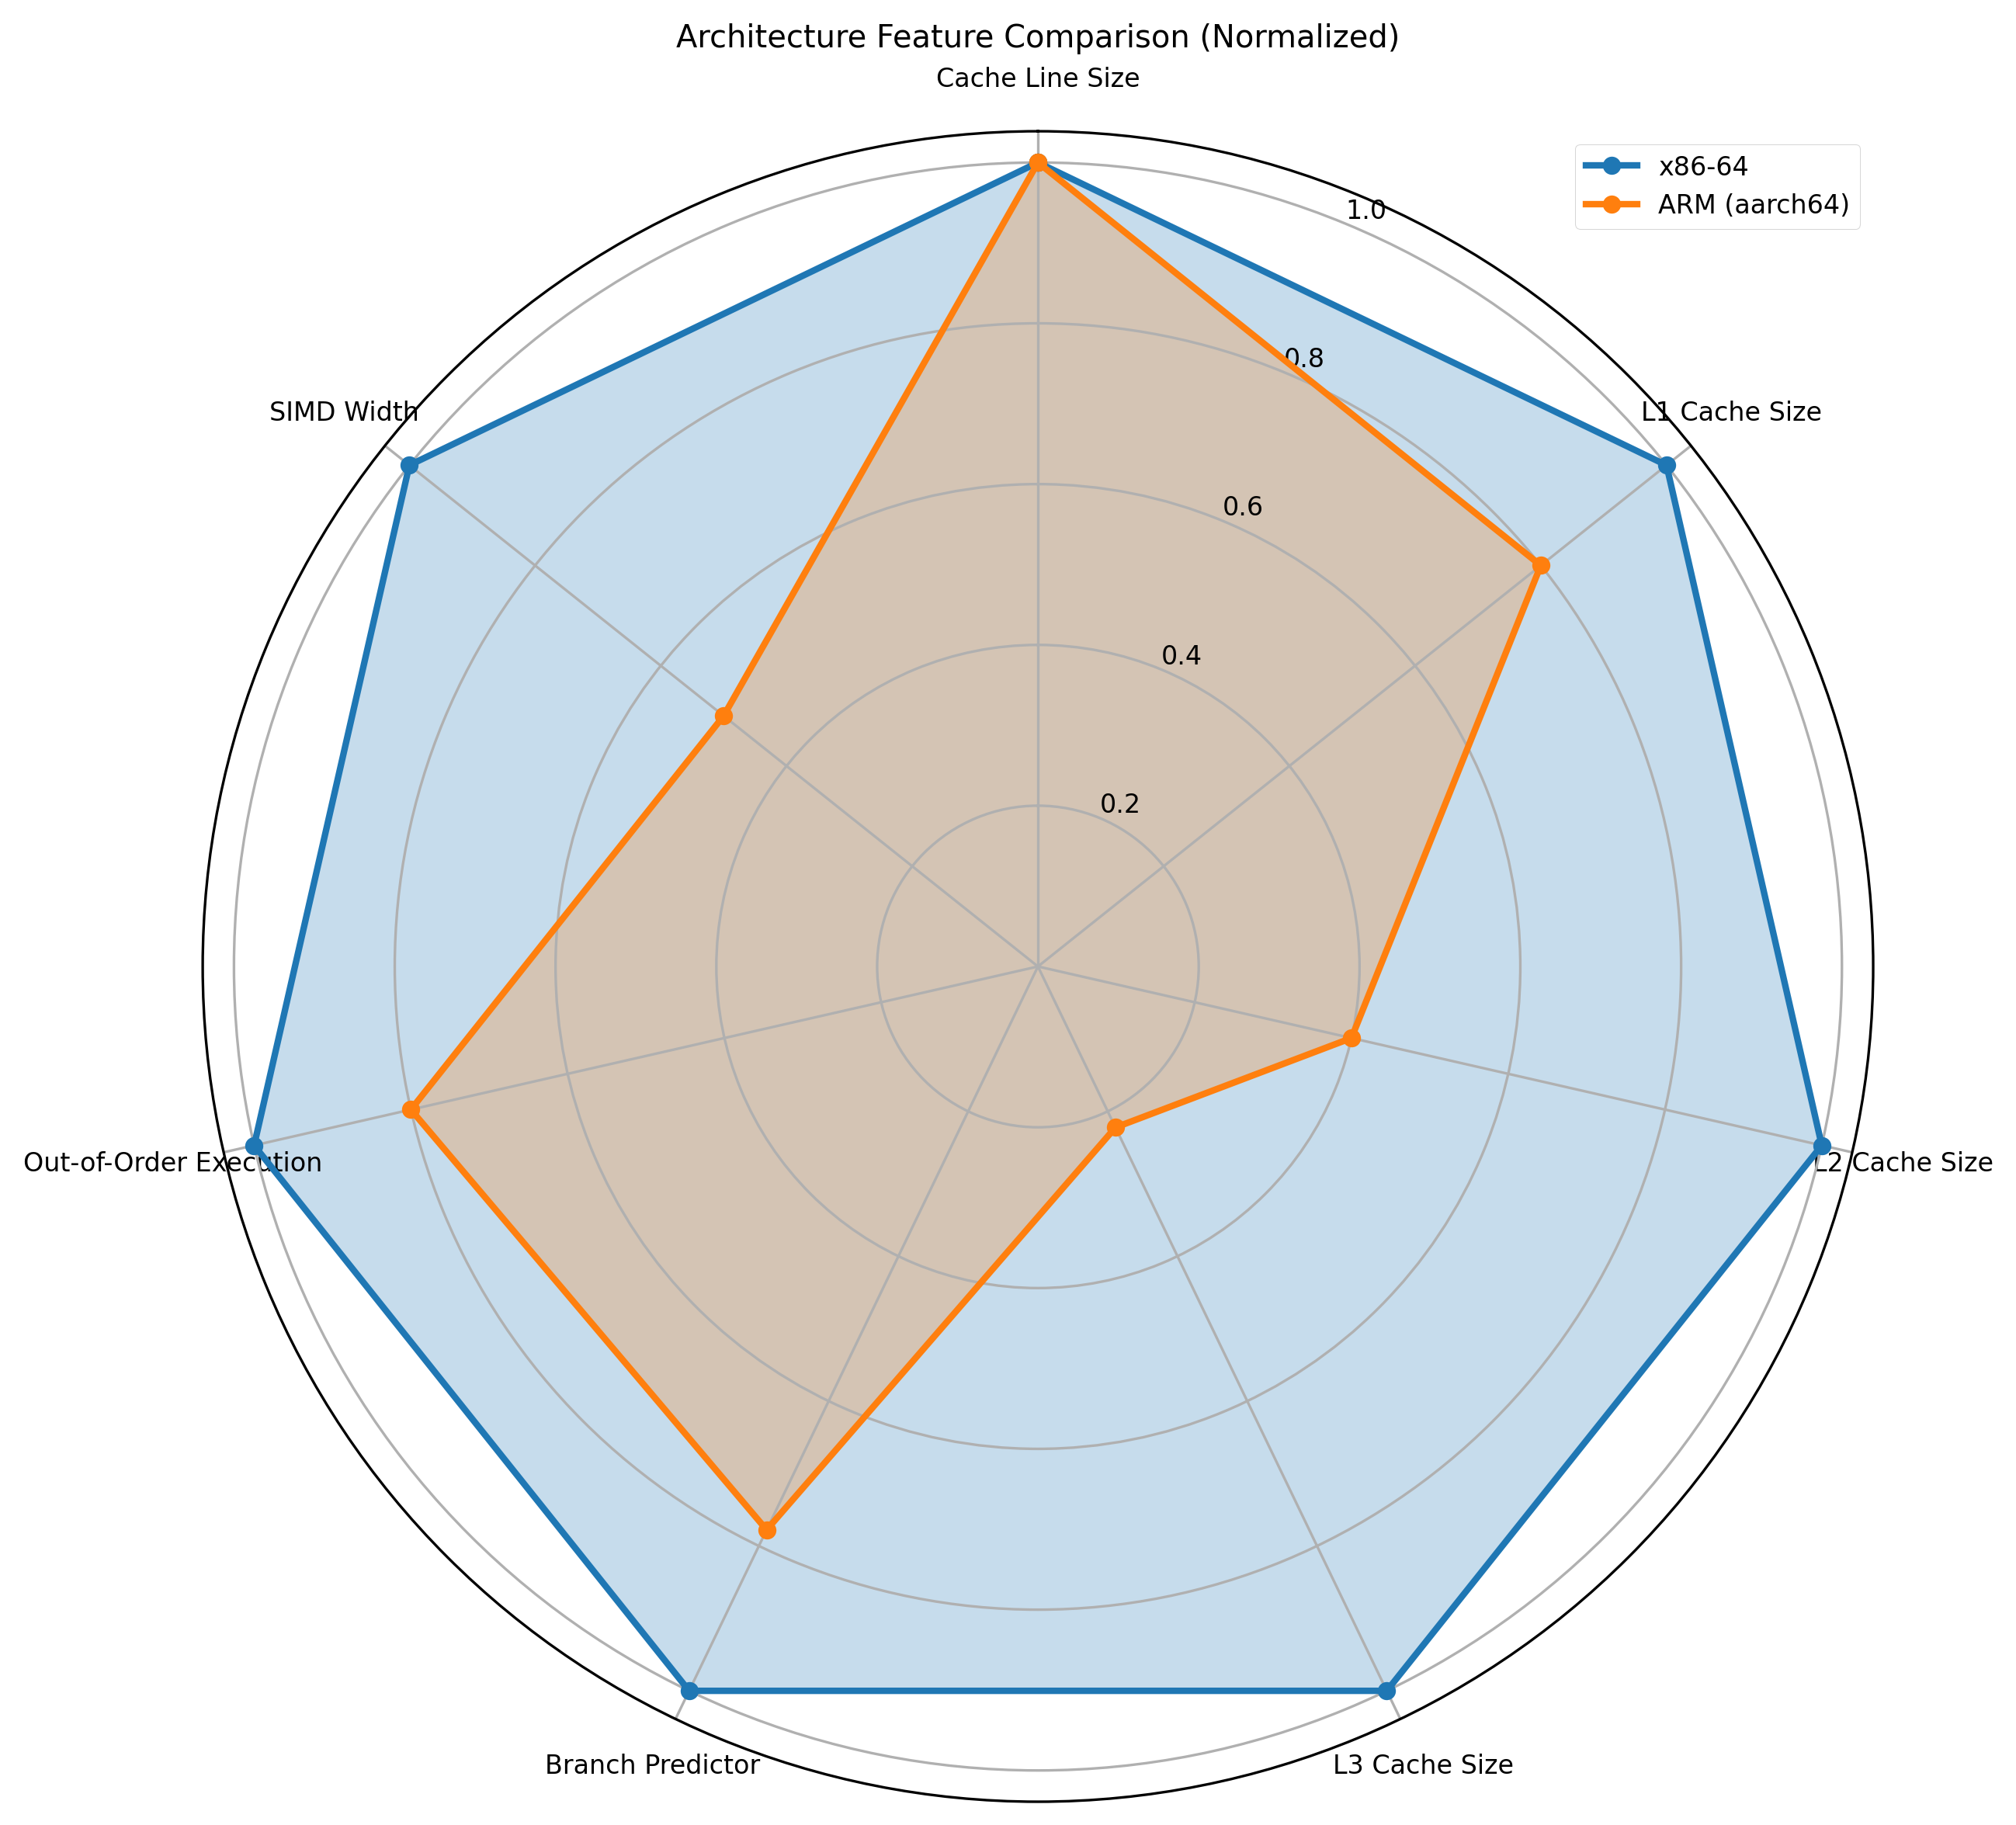
\includegraphics[width=\textwidth]{architecture_comparison.png}
    \caption{硬件架构比较雷达图}
    \label{fig:hardware_config}
  \end{subfigure}
  \hfill
  \begin{subfigure}[b]{0.48\textwidth}
    \centering
    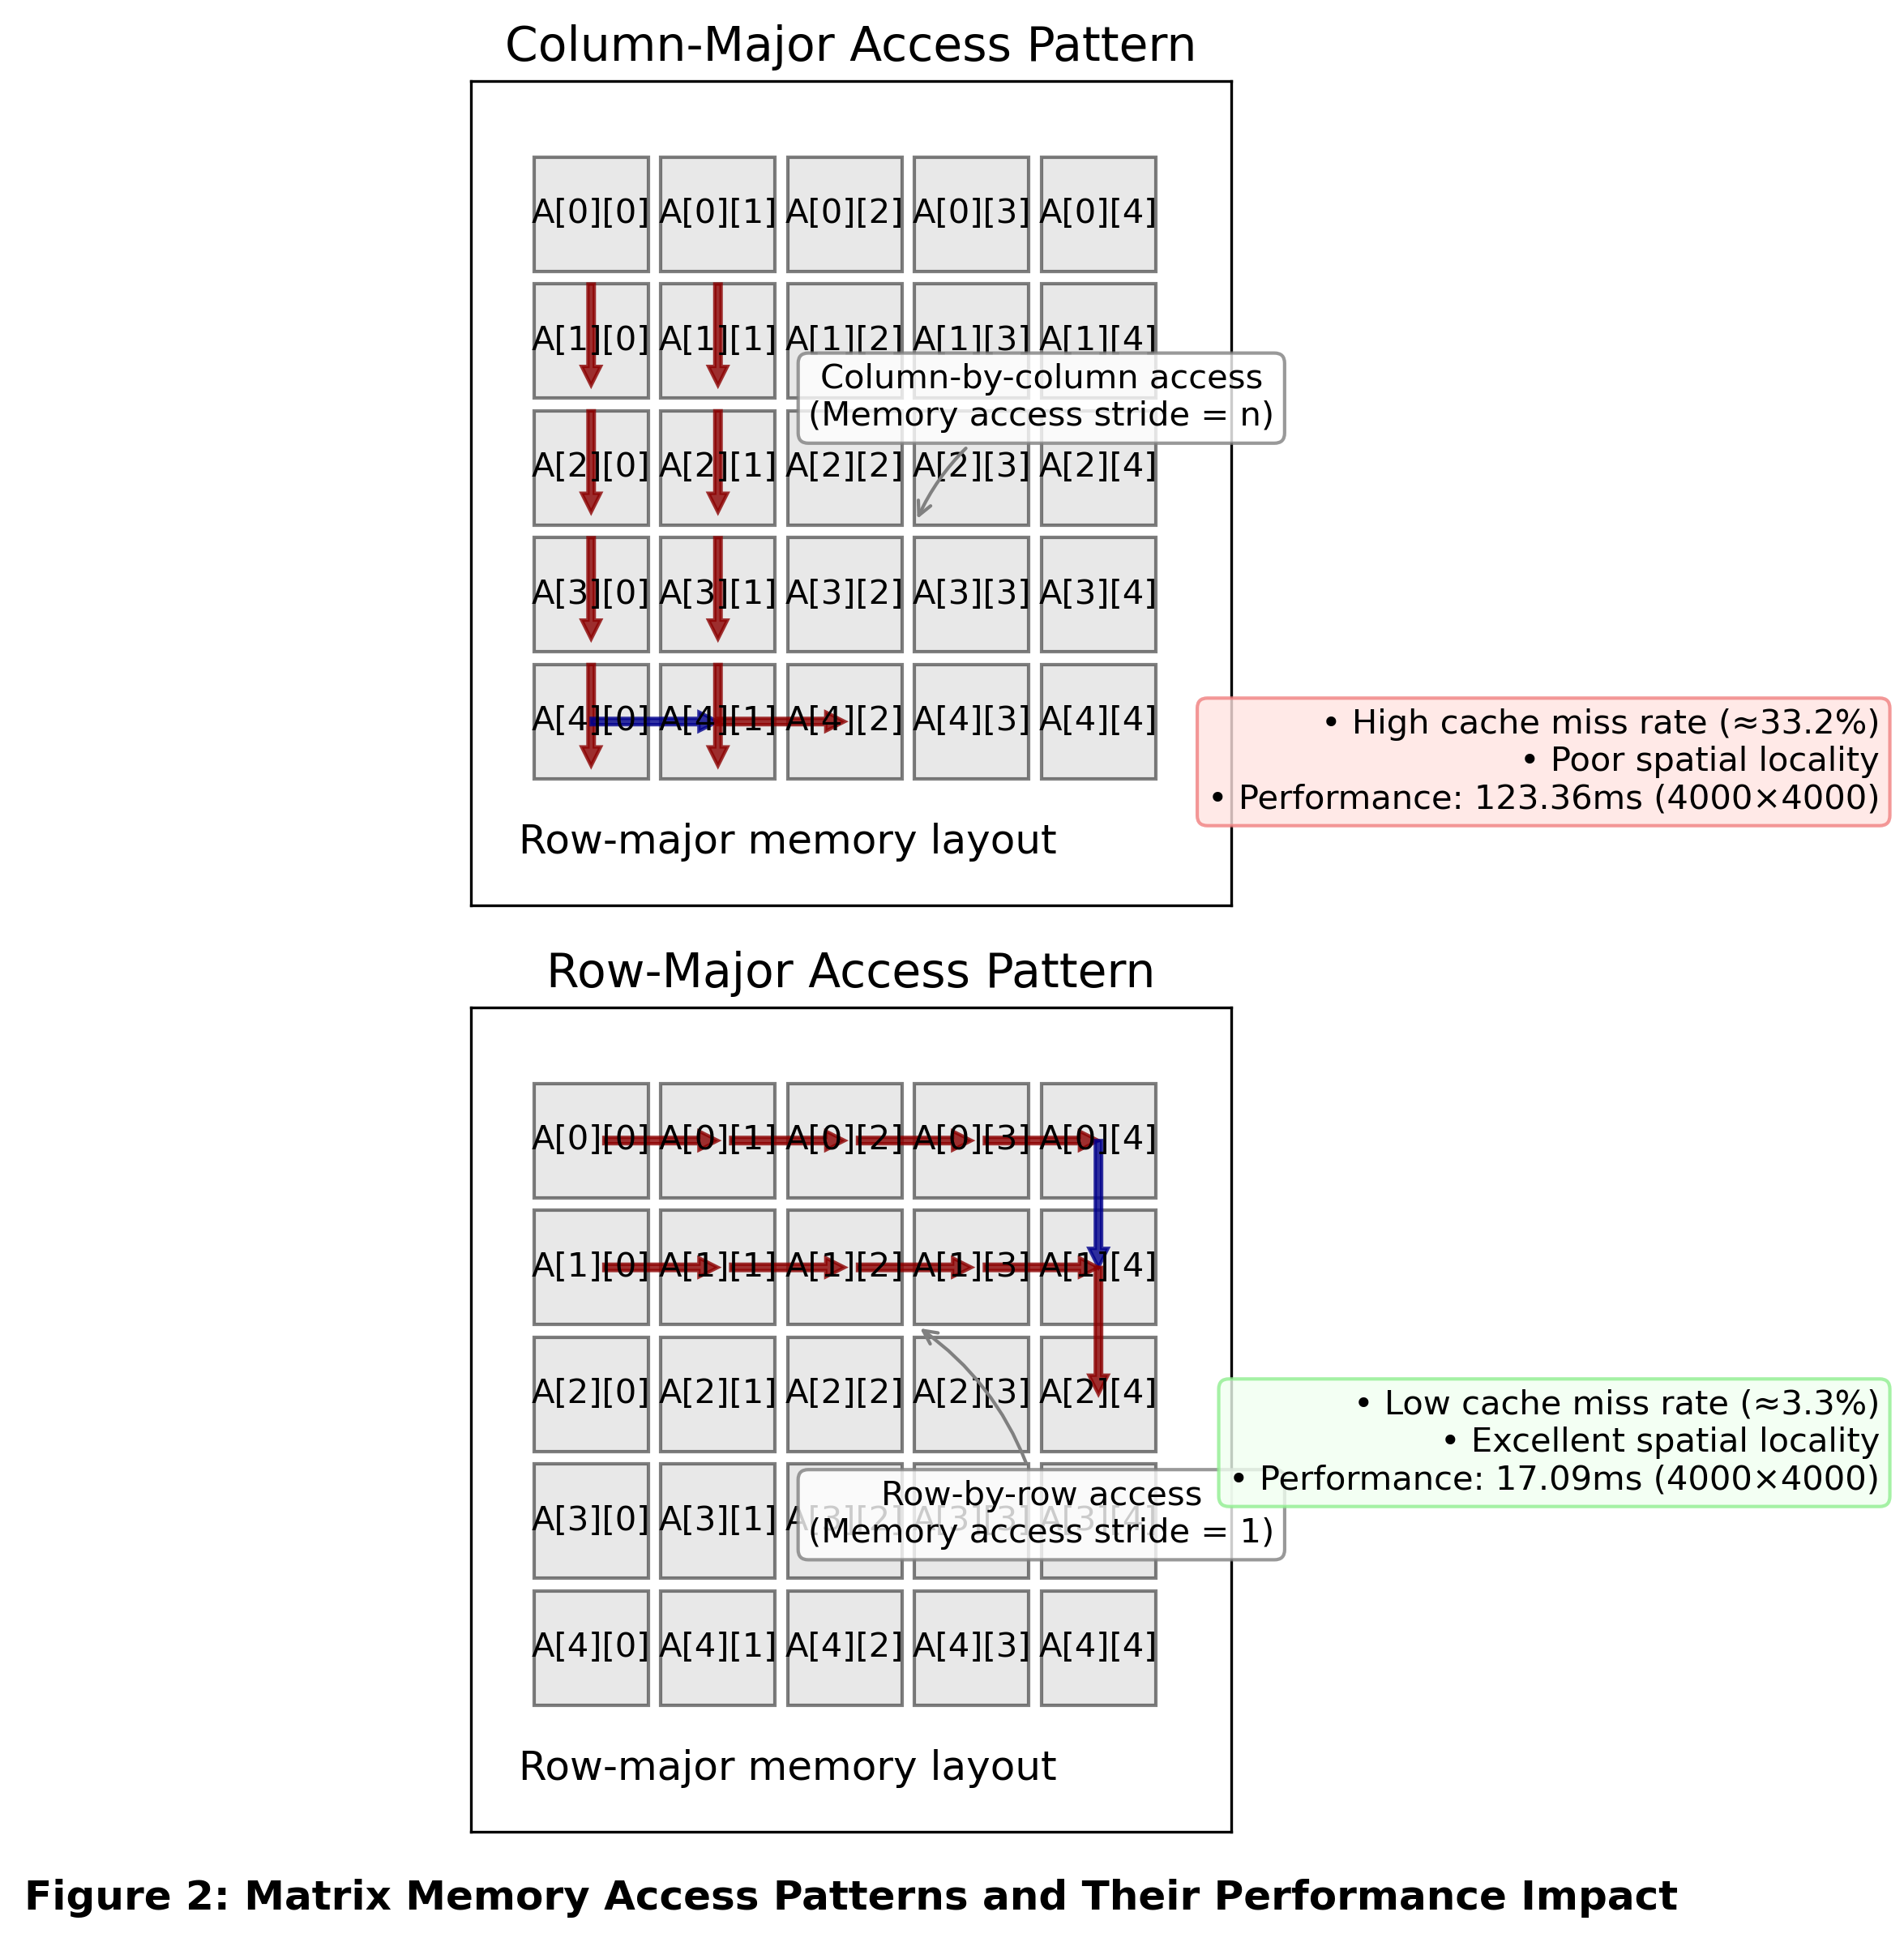
\includegraphics[width=\textwidth]{access_patterns_diagram.png}
    \caption{访问模式示意图}
    \label{fig:access_patterns}
  \end{subfigure}
  \caption{硬件架构与访问模式分析}
  \label{fig:hardware_access}
\end{figure}

\textbf{图1 架构特性雷达图}:展示了x86-64与ARM aarch64架构在多个性能指标上的相对强弱。x86-64在缓存大小、乱序执行能力和SIMD宽度等方面具有明显优势,有利于指令级并行和向量化计算;ARM架构虽然在这些指标上较低,但设计更为平衡。两者共同特点是相同的缓存行大小(64字节),表明针对空间局部性的优化策略在两种架构上都有效。该图直观展示了为什么某些优化在不同架构上效果有差异。

\textbf{图2 矩阵访问模式示意图}:直观展示了两种不同的矩阵访问模式及其对性能的影响。上图为列优先访问方式,在C/C++行优先存储的内存布局下,导致内存访问跨度大(stride=n),缓存未命中率高达33.2\%,4000x4000矩阵上执行时间达123.36ms;下图为行优先访问方式,访问顺序与内存存储顺序一致(stride=1),充分利用空间局部性,缓存未命中率仅为3.3\%,同样大小的矩阵计算仅需17.09ms。红色箭头表示主要访问路径,蓝色箭头表示转换到下一行/列的路径。这一可视化解释了为什么内存访问模式对性能影响如此显著。

\subsection{软件环境}

\begin{itemize}
  \item \textbf{编译器}:GCC 13.3.0
  \item \textbf{编译选项}:-O0/-O2/-O3, ARM交叉编译使用aarch64-linux-gnu-g++
  \item \textbf{性能分析}:Valgrind Cachegrind
  \item \textbf{数据处理}:Python 3.10 (numpy, pandas, matplotlib)
\end{itemize}

\section{实验一:n×n矩阵与向量内积}

\subsection{算法设计}

\subsubsection{平凡算法设计思路}

平凡算法采用列优先访问方式计算矩阵与向量的内积。对于n×n的矩阵A和长度为n的向量x,结果向量y的计算公式为:

\begin{equation}
  y[i] = \sum_{j=0}^{n-1} A[i][j] \times x[j]
\end{equation}

列优先访问实现代码:

\begin{lstlisting}[language=C++]
void col_access(const std::vector<std::vector<double>>& matrix, 
               const std::vector<double>& vector,
               std::vector<double>& result) {
    int n = matrix.size();
    for (int j = 0; j < n; j++) {  // 列优先访问
        for (int i = 0; i < n; i++) {
            result[i] += matrix[i][j] * vector[j];
        }
    }
}
\end{lstlisting}

这种方式在访问矩阵元素时,由于C/C++中二维数组按行存储的特性,会导致大步幅访问,相邻两次访问的\verb|matrix[i][j]|和\verb|matrix[i+1][j]|在内存中相距n个元素,导致频繁的缓存缺失。

\subsubsection{cache优化算法设计思路}

行优先访问和循环展开优化代码:

\begin{lstlisting}[language=C++]
void row_access(const std::vector<std::vector<double>>& matrix, 
               const std::vector<double>& vector,
               std::vector<double>& result) {
    int n = matrix.size();
    for (int i = 0; i < n; i++) {  // 行优先访问
        double sum = 0.0;
        for (int j = 0; j < n; j++) {
            sum += matrix[i][j] * vector[j];
        }
        result[i] = sum;
    }
}

void unroll10(const std::vector<std::vector<double>>& matrix, 
            const std::vector<double>& vector,
            std::vector<double>& result) {
    int n = matrix.size();
    for (int i = 0; i < n; i++) {
        double sum = 0.0;
        int j = 0;
        for (; j <= n - 10; j += 10) {
            sum += matrix[i][j] * vector[j] +
                   matrix[i][j+1] * vector[j+1] +
                   matrix[i][j+2] * vector[j+2] +
                   matrix[i][j+3] * vector[j+3] +
                   matrix[i][j+4] * vector[j+4];
        }
        for (; j < n; j++) {
            sum += matrix[i][j] * vector[j];
        }
        result[i] = sum;
    }
}
\end{lstlisting}

\subsection{性能测试}

测量结果表明,行优先访问在各矩阵大小上都比列优先访问快约7-12倍,循环展开可进一步提升性能。在4000x4000矩阵上,列访问耗时123.36ms,行访问降至17.09ms,Unroll10进一步优化至10.13ms。

\begin{figure}[htbp]
  \centering
  \begin{subfigure}[b]{0.45\textwidth}
    \centering
    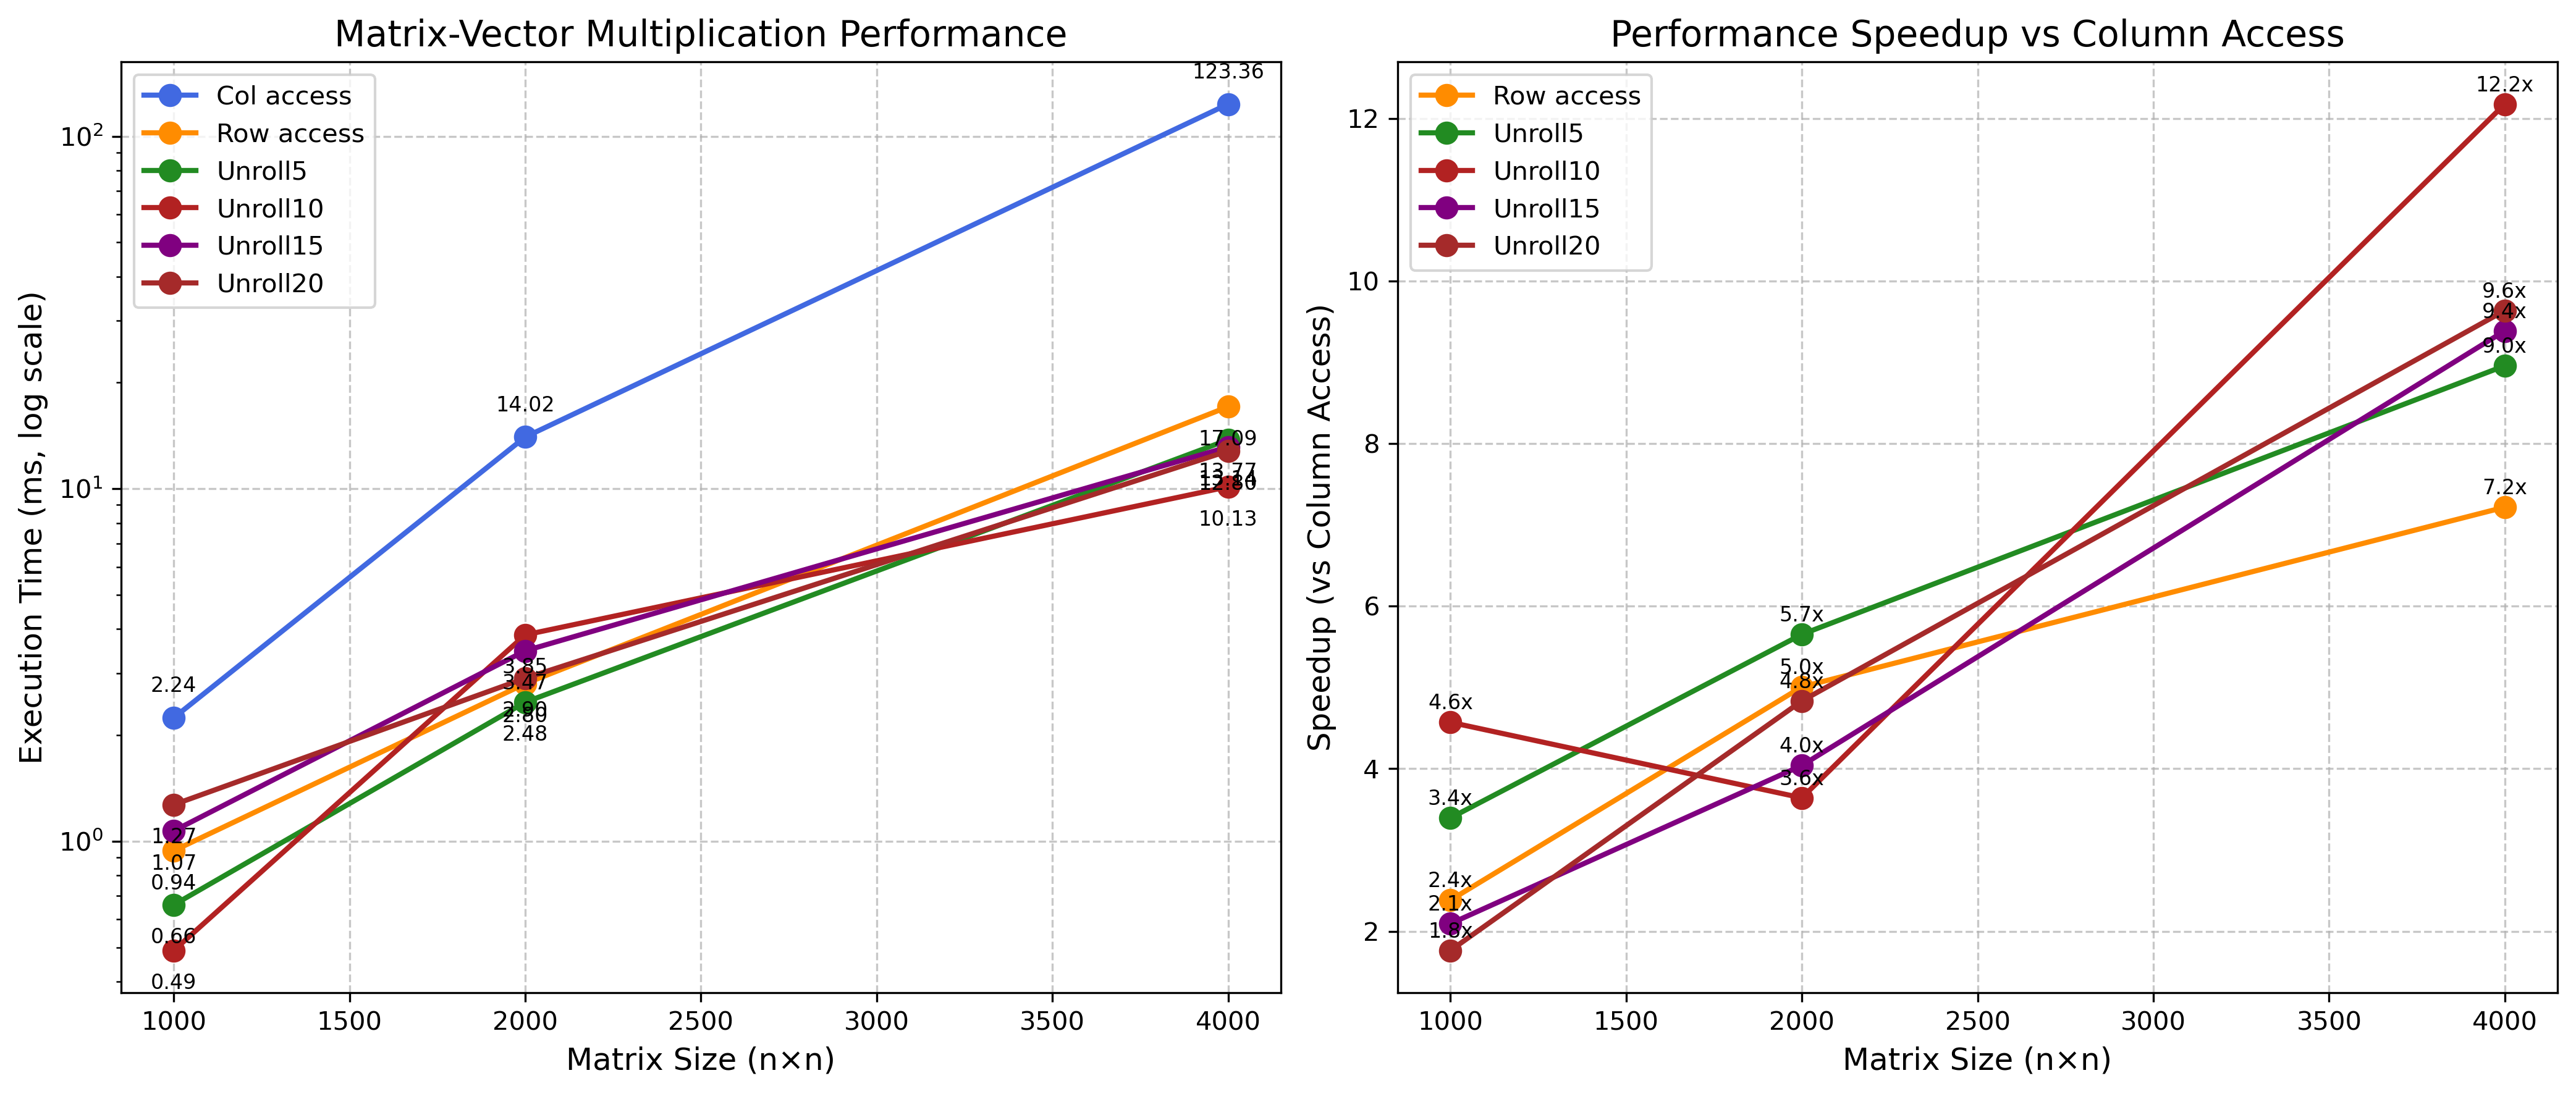
\includegraphics[width=\textwidth]{matrix_vector_performance.png}
    \caption{矩阵向量乘法性能比较}
    \label{fig:matrix_vector_performance}
  \end{subfigure}
  \hfill
  \begin{subfigure}[b]{0.45\textwidth}
    \centering
    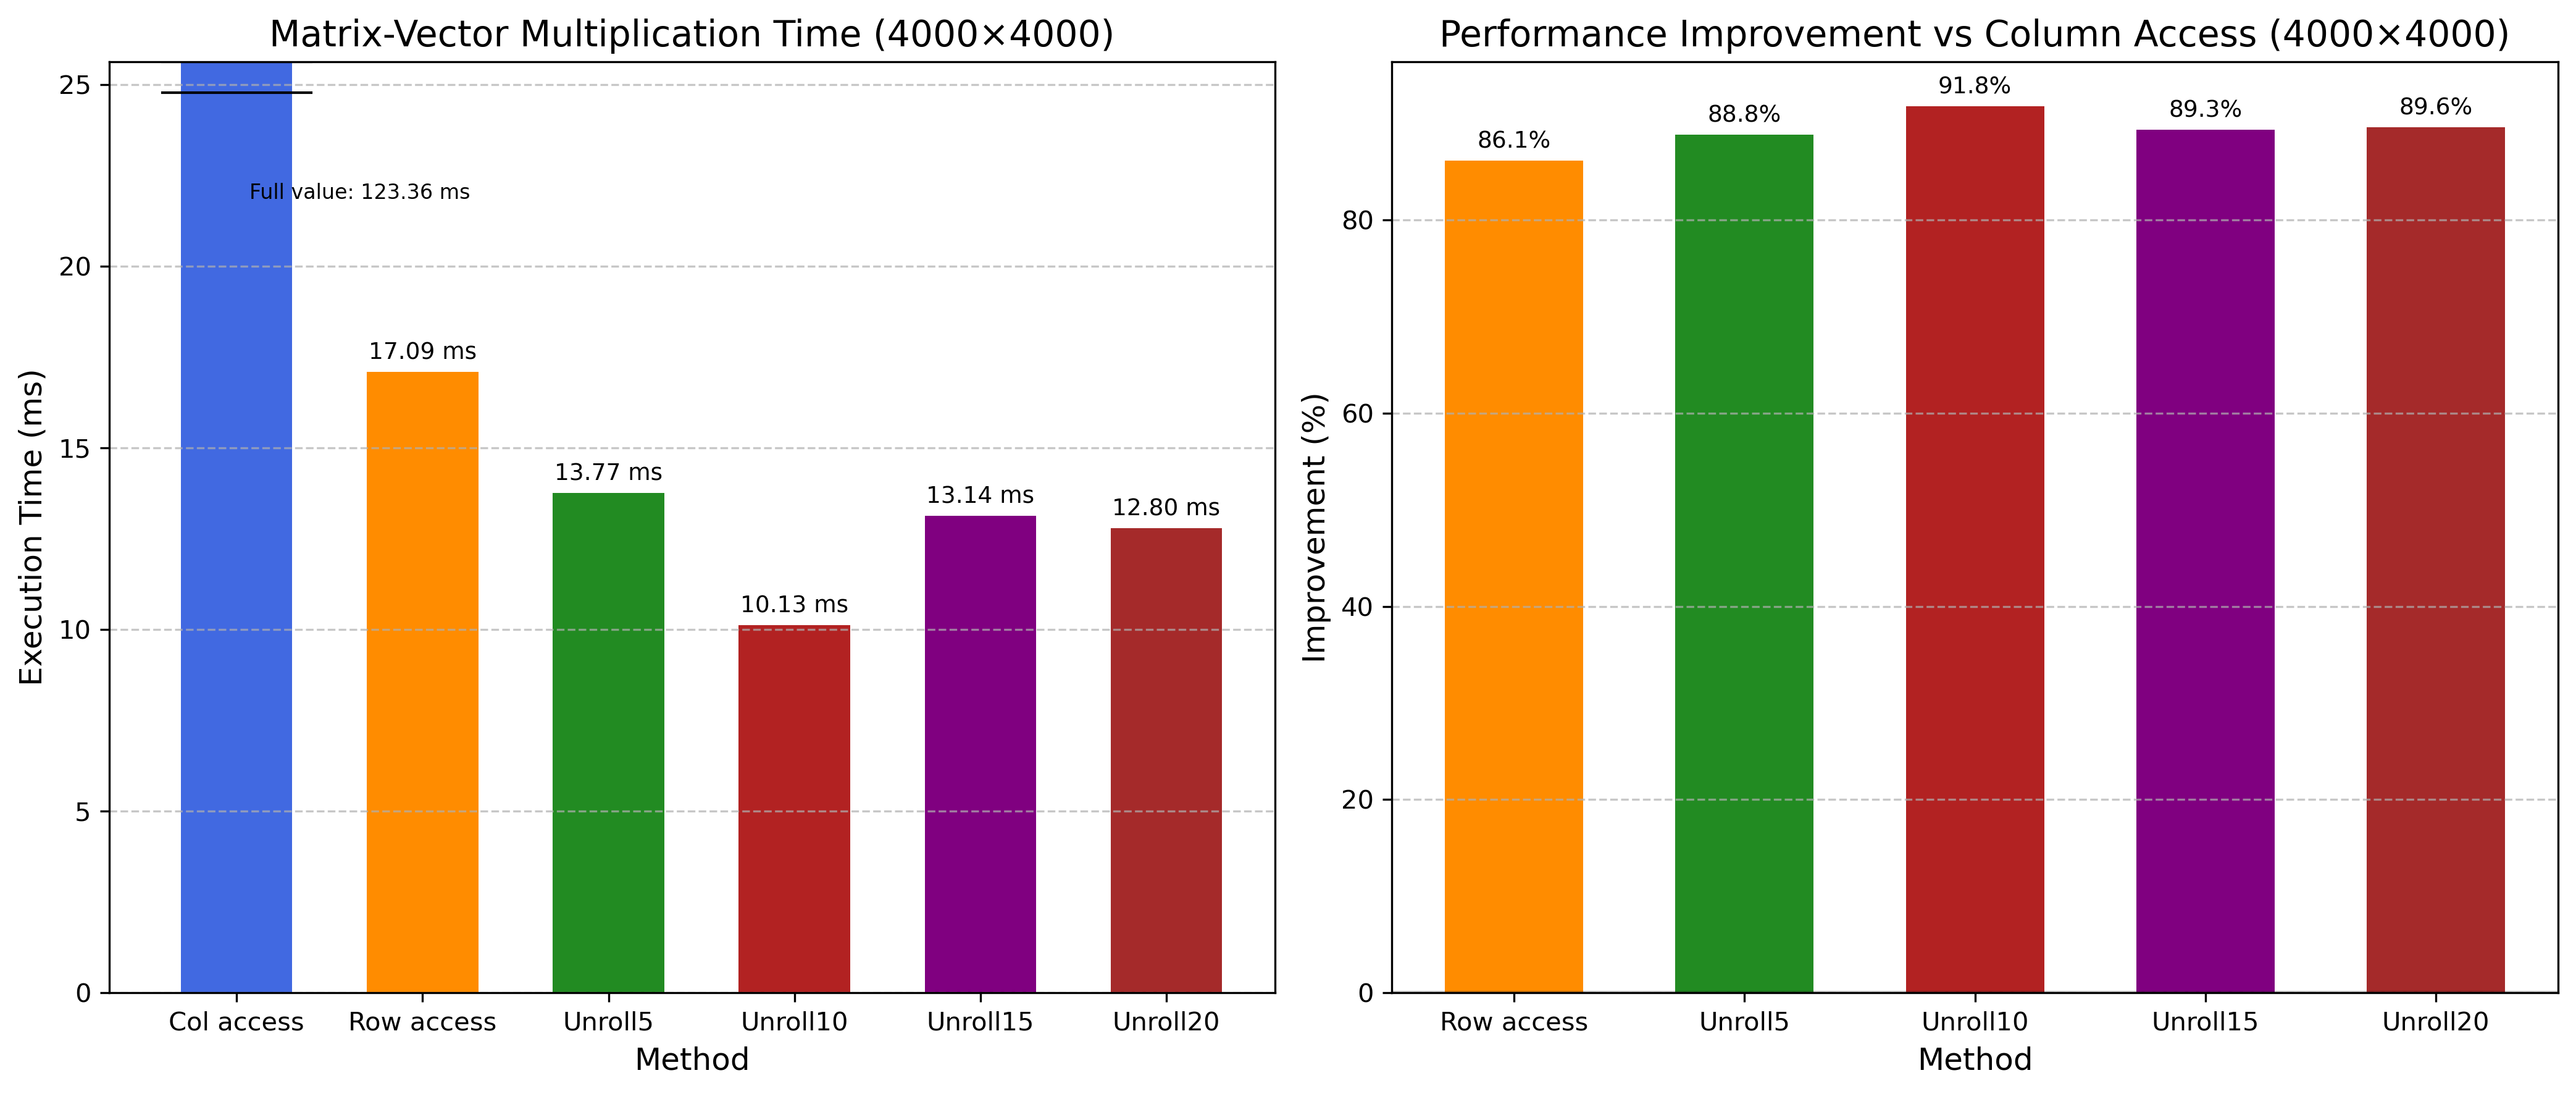
\includegraphics[width=\textwidth]{matrix_vector_detail_performance.png}
    \caption{详细性能对比}
    \label{fig:detail_performance}
  \end{subfigure}
  \caption{矩阵向量乘法实验结果}
  \label{fig:matrix_results}
\end{figure}

\textbf{图3 矩阵-向量乘法性能}:左图展示了不同算法在各矩阵尺寸下的执行时间(对数刻度),右图展示了相对于列访问的加速比。数据显示:(1) 矩阵规模增大时,列访问性能下降最快,4000x4000矩阵时达到123.36ms;(2) 行访问通过优化空间局部性将执行时间降至17.09ms,加速比为7.2倍;(3) Unroll10算法在所有矩阵尺寸上都表现最佳,4000x4000矩阵上达到12.2倍加速比;(4) 随着矩阵规模增大,空间局部性优化的效果更为显著,这与理论预期一致。这表明内存访问模式对性能的影响随问题规模增大而更加突出。

\textbf{图4 详细性能对比}:左图展示4000x4000矩阵上各算法的执行时间,右图展示相对于列访问的性能提升百分比。数据表明:(1) 列访问是最慢的(123.36ms);(2) 行访问降低86.1\%至17.09ms;(3) Unroll10表现最佳,执行时间仅为10.13ms,相比列访问提升了91.8\%;(4) 所有优化方法都获得了显著提升,即使最小的改进(Unroll15)也比列访问快89.4\%。这证明了针对特定硬件架构的优化策略能够带来显著性能收益。

\subsubsection{编译器优化影响}

\begin{figure}[ht]
  \centering
  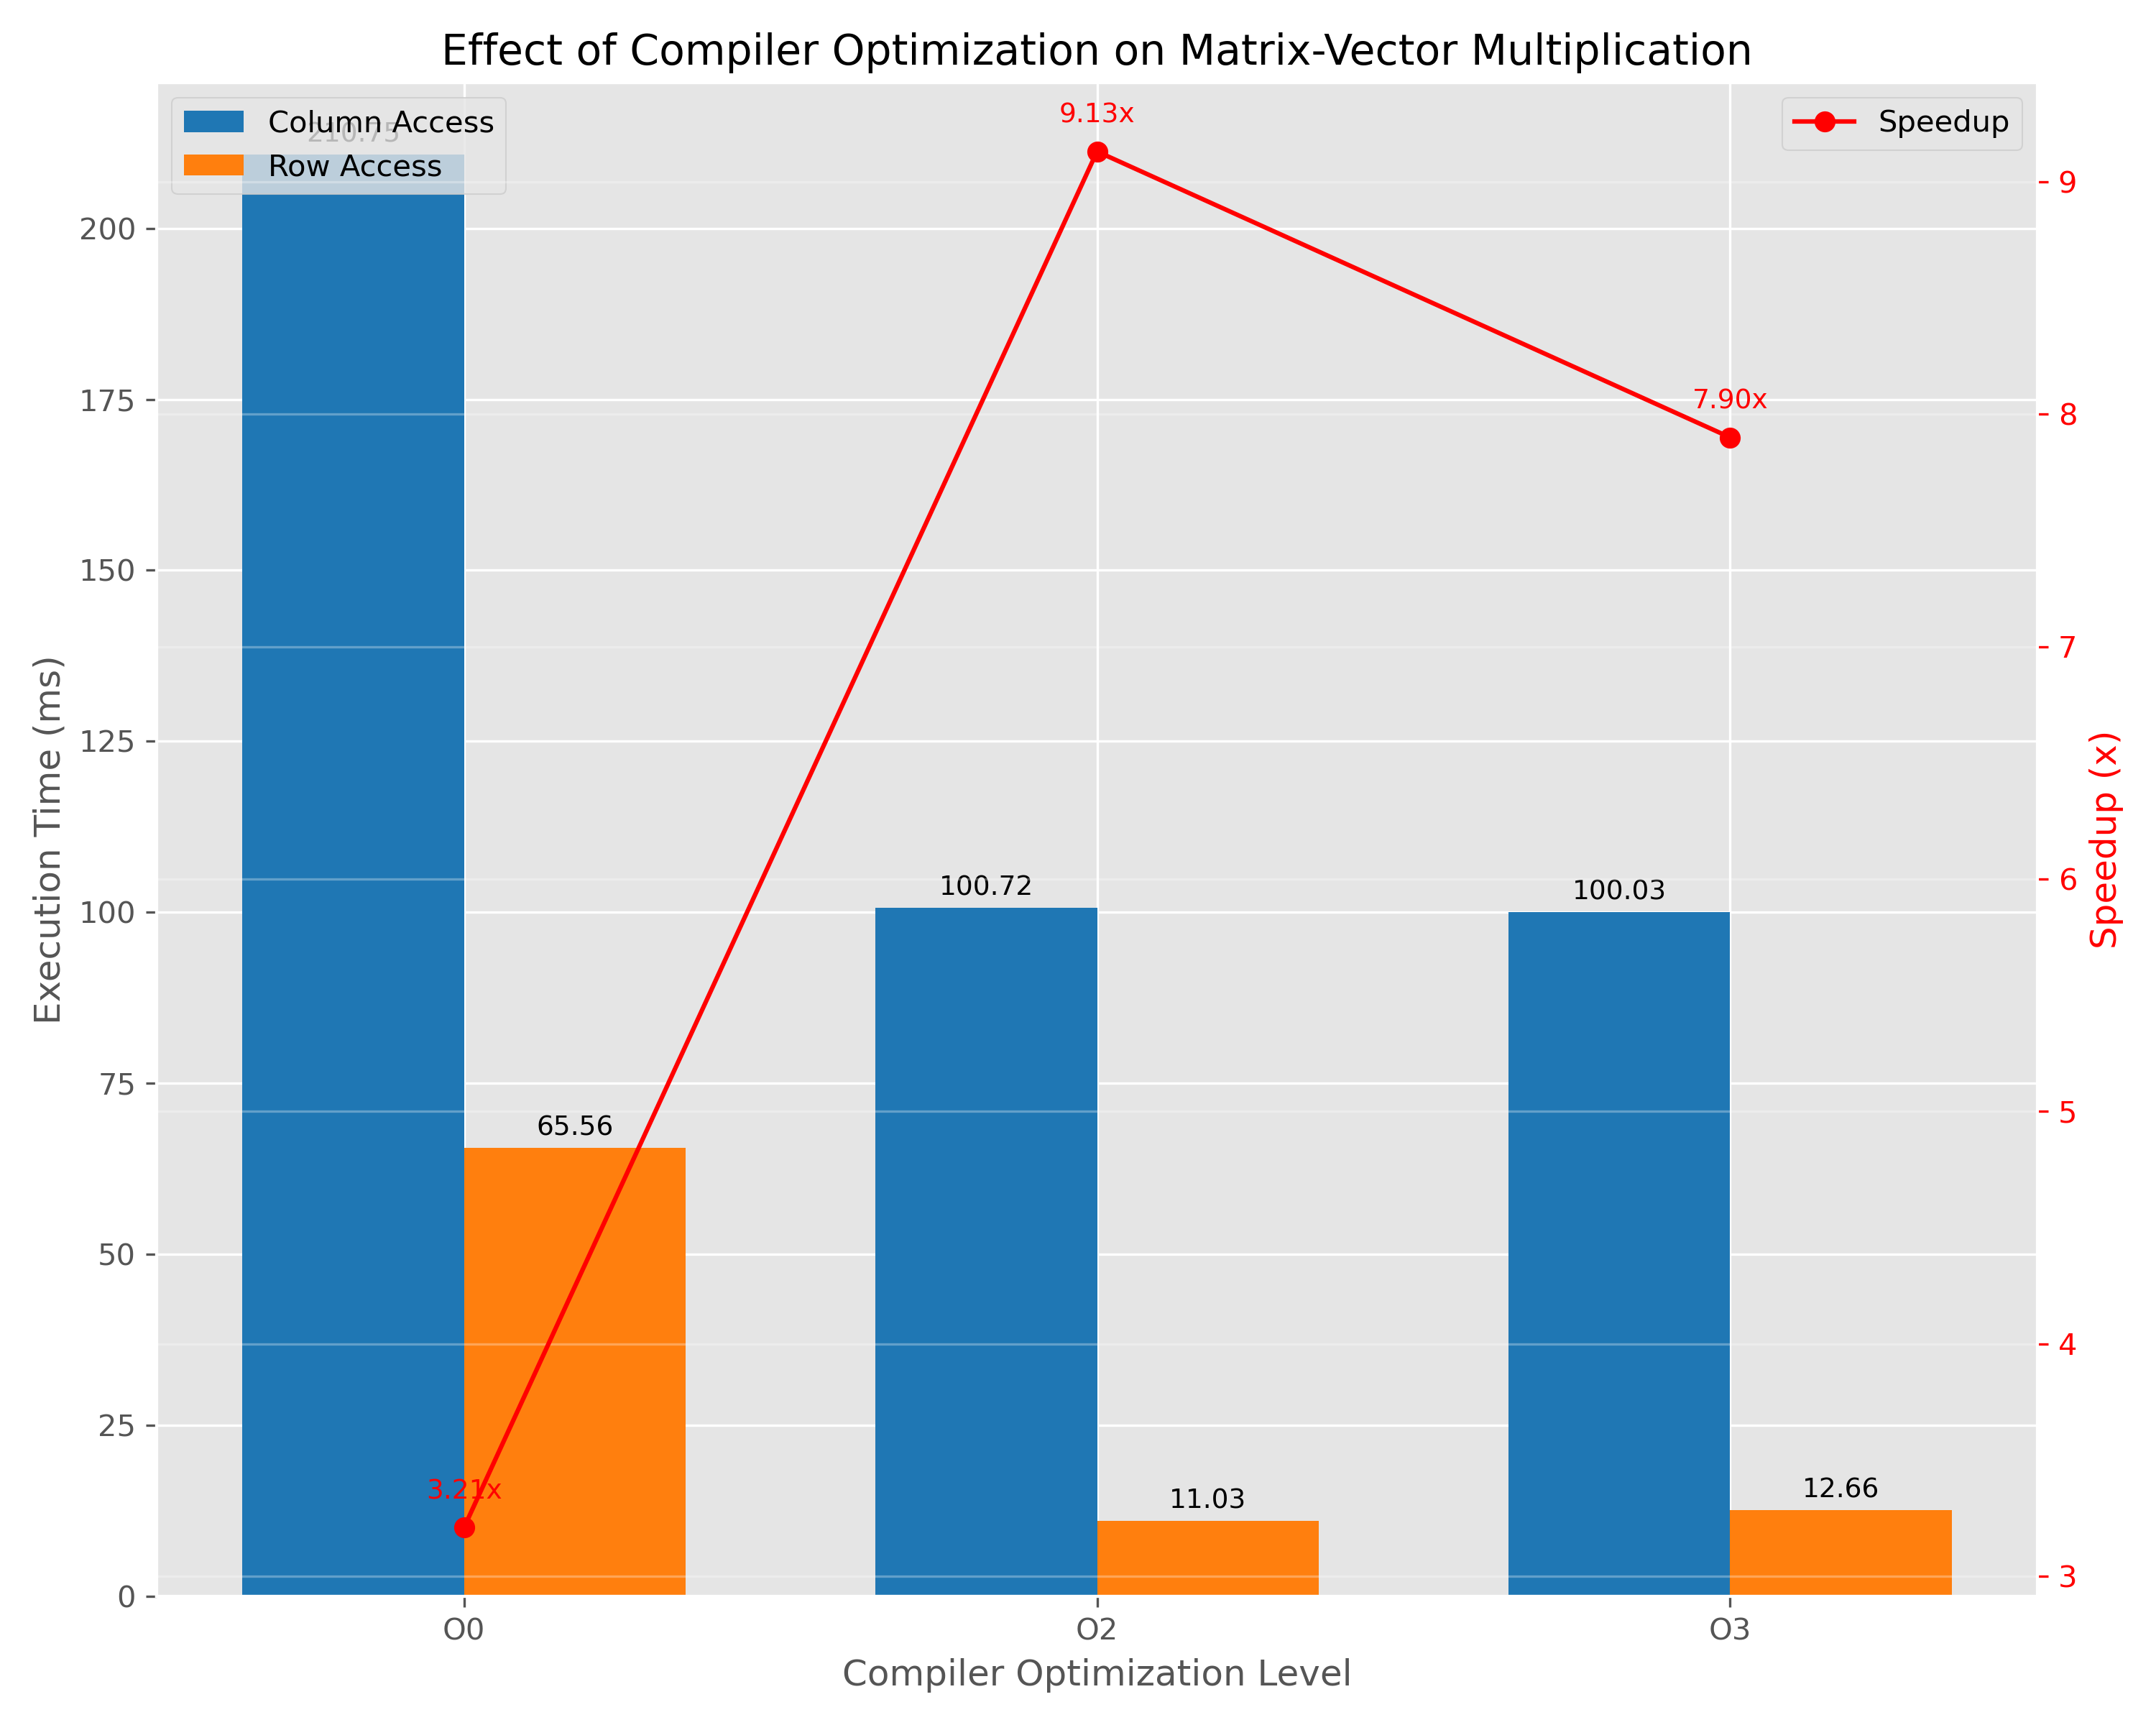
\includegraphics[width=0.45\textwidth]{compiler_opt_matrix.png}
  \caption{编译器优化对矩阵乘法的影响}
  \label{fig:compiler_opt_matrix}
\end{figure}

\textbf{图7 编译器优化级别影响}:展示了不同编译优化级别对矩阵计算性能的影响。无优化(O0)时列访问耗时225.64ms,行访问65.56ms;O3优化后分别提升至100.03ms和12.66ms。红线加速比走势表明编译器优化开始能提高加速比,在O2达到最高的9.13,但之后开始下降。这可能是因为O3级别下编译器对列访问模式进行了更激进的优化,缩小了与行访问之间的相对差距。这说明编译器优化虽然重要,但不能完全弥补算法设计中的本质缺陷。

\subsection{profiling}

\subsubsection{平凡算法}

使用Cachegrind分析平凡算法(列优先访问)的缓存性能:L1缓存未命中率约33.2\%,主要发生在内层循环访问\verb|matrix[i][j]|时,由于列优先访问导致的跨行访问,每次访问大概率会触发新的缓存行加载。

\subsubsection{cache优化算法}

行优先访问的缓存性能显著改善:L1缓存未命中率仅约3.3\%,缓存行利用率高,一次加载的缓存行中的多个元素会被连续使用。循环展开效果分析显示Unroll10展开级别在4000x4000矩阵上性能最佳,比基础行访问提升约40.7\%。

\begin{figure}[htbp]
  \centering
  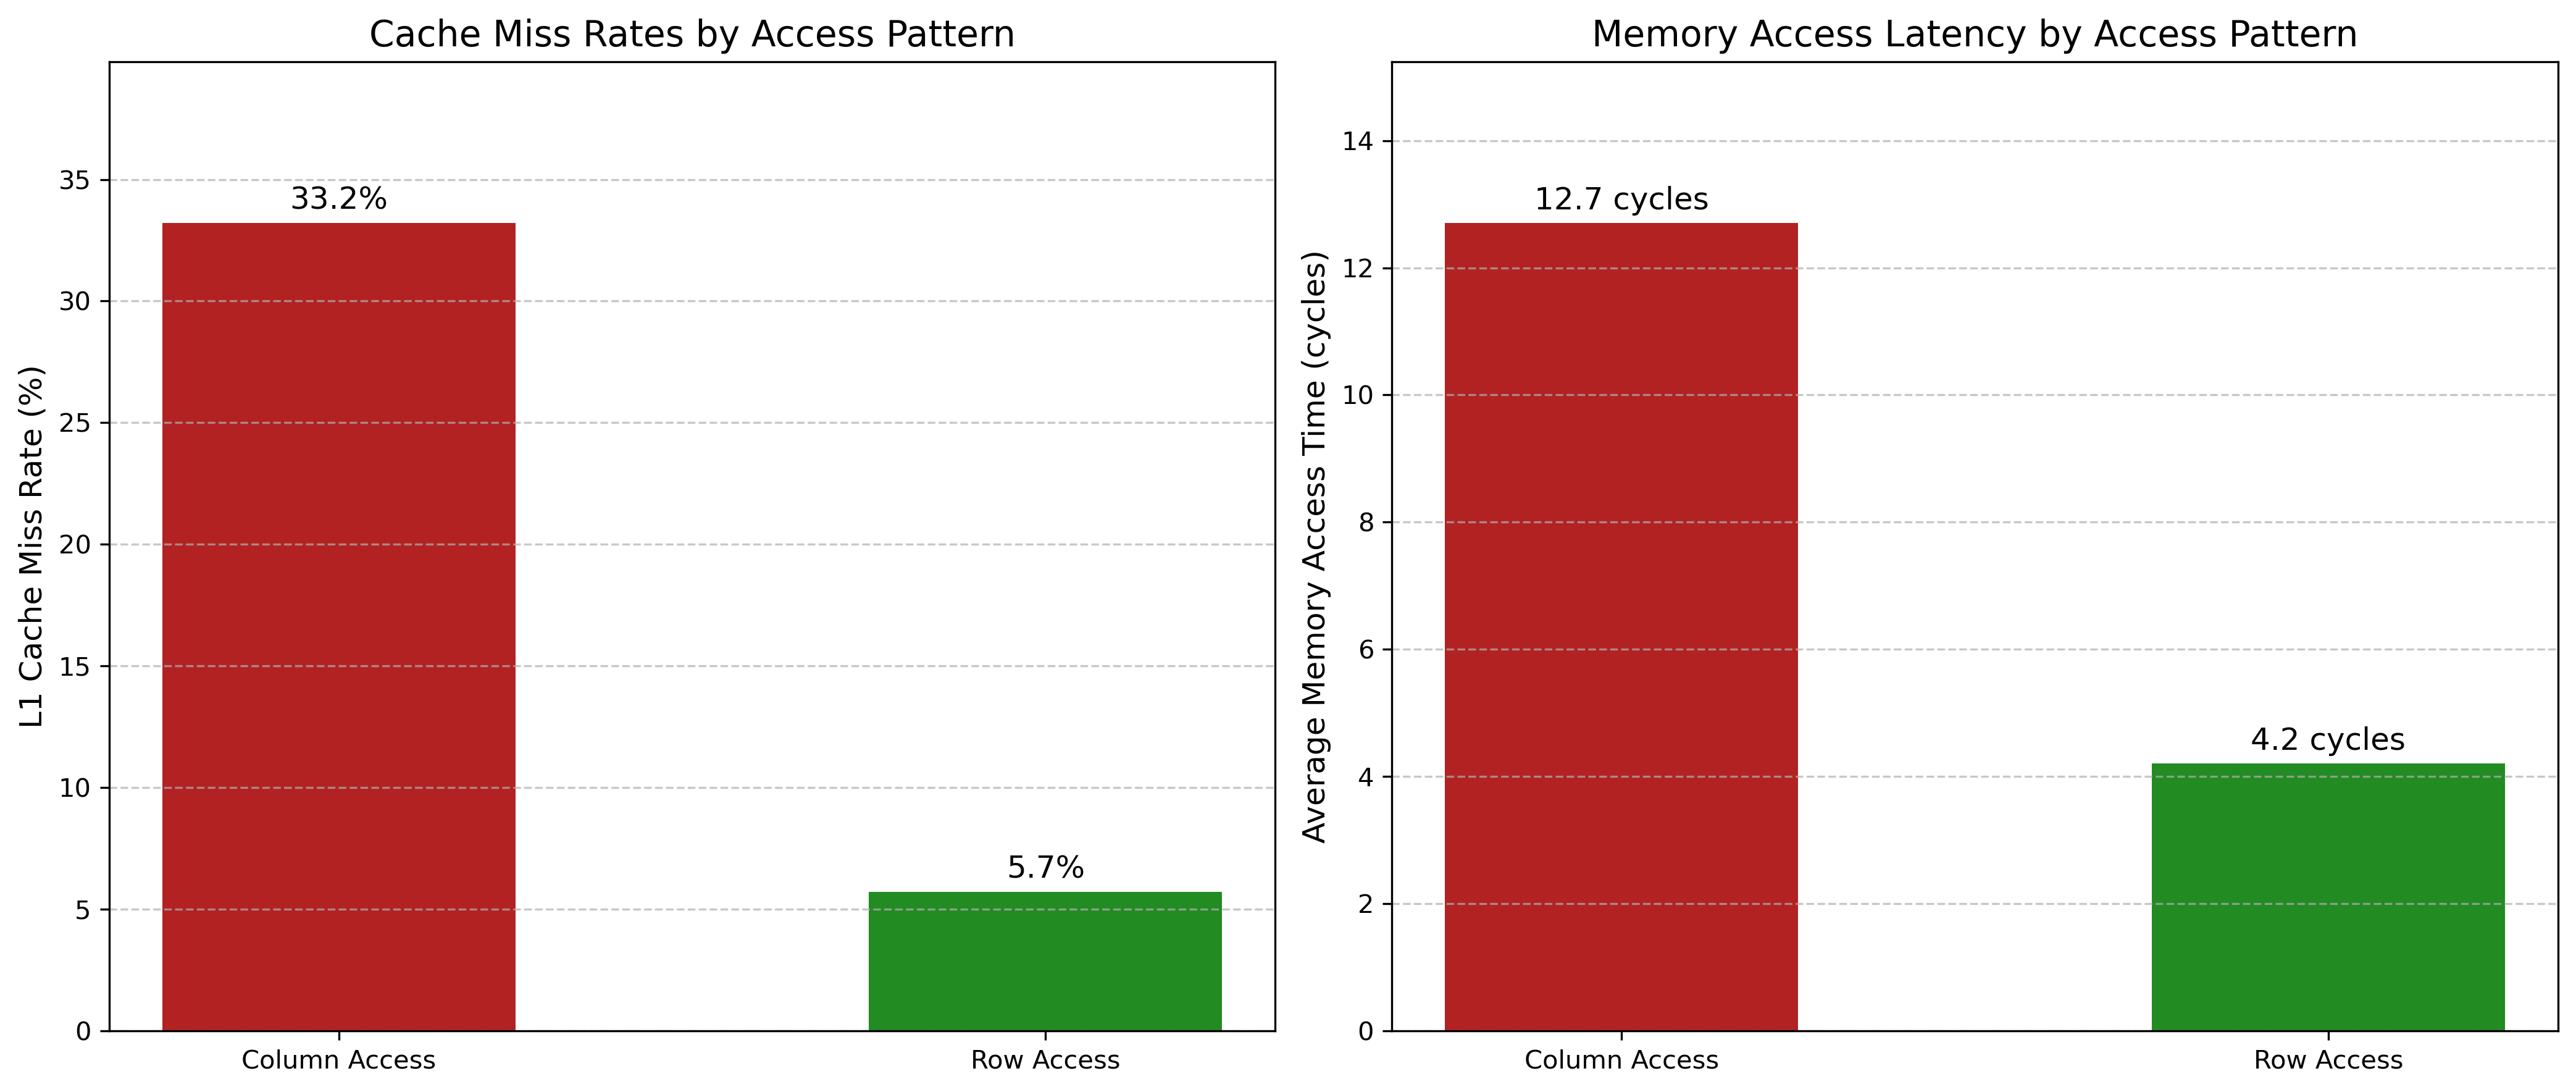
\includegraphics[width=0.45\textwidth]{cache_miss_analysis.png}
  \caption{缓存未命中分析}
  \label{fig:cache_miss}
\end{figure}

\textbf{图5 缓存未命中分析}:左图对比了列访问和行访问的L1缓存未命中率,列访问的未命中率(33.2\%)显著高于行访问(3.3\%);右图展示了平均内存访问延迟,列访问(12.7周期)远高于行访问(4.2周期),这直接解释了列访问性能差的原因。这一数据从底层硬件角度验证了性能差异的根本原因。

\subsection{架构对比分析}

\begin{figure}[htbp]
  \centering
  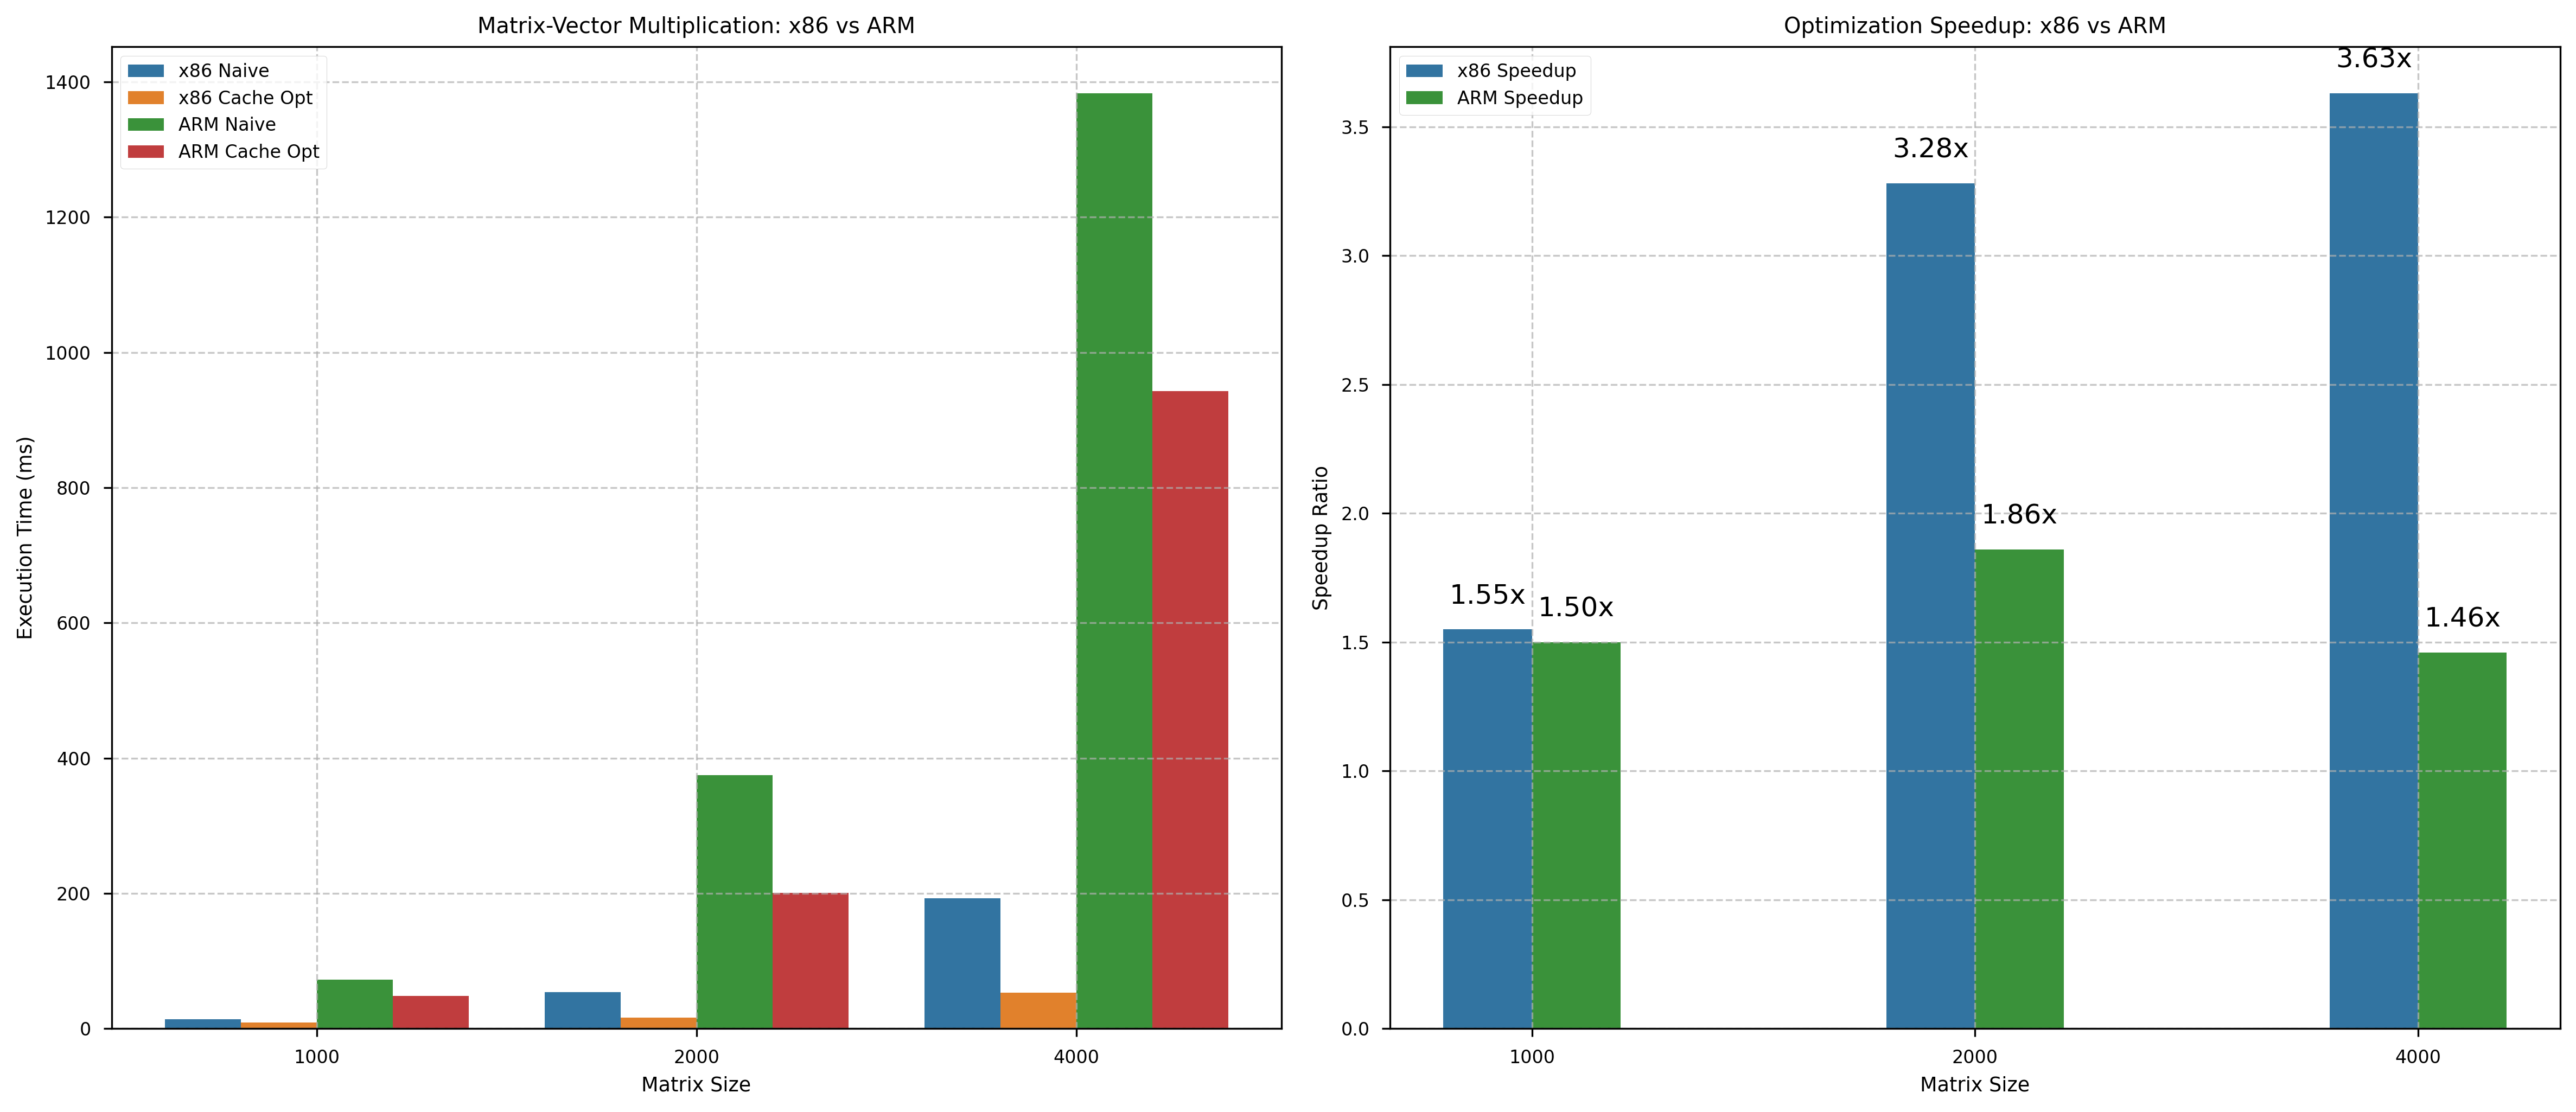
\includegraphics[width=0.45\textwidth]{matrix_arch_comparison.png}
  \caption{x86与ARM架构性能对比}
  \label{fig:arch_comparison}
\end{figure}

x86架构上缓存优化的收益在大矩阵(4000x4000)上更高(3.63倍),而ARM架构上加速比随矩阵增大先提高后下降,在2000x2000矩阵上达到最高的1.86倍。这一现象可能是由于ARM架构的较小缓存容量(L2:512KB,L3:4MB)在处理4000x4000矩阵时已经饱和,导致即使是行访问模式也无法完全避免频繁的缓存替换。如图\ref{fig:arch_comparison}所示。

\section{实验二:n个数求和}

\subsection{算法设计}

\subsubsection{平凡算法设计思路}

平凡算法采用简单的顺序求和方式:

\begin{lstlisting}[language=C++]
double naive_sum(const std::vector<double>& array) {
    double sum = 0.0;
    for (size_t i = 0; i < array.size(); ++i) {
        sum += array[i];
    }
    return sum;
}
\end{lstlisting}

此算法有良好的空间局部性,但存在严重的数据依赖。

\subsubsection{超标量优化算法设计思路}

双链路算法通过创建两个独立的累加路径,让处理器能够同时执行两个独立的累加操作:

\begin{lstlisting}[language=C++]
double dual_path_sum(const std::vector<double>& array) {
    double sum1 = 0.0, sum2 = 0.0;
    size_t n = array.size();
    for (size_t i = 0; i < n; i += 2) {
        sum1 += array[i];
        if (i + 1 < n) sum2 += array[i + 1];
    }
    return sum1 + sum2;
}
\end{lstlisting}

\subsection{性能测试}

实际测量结果表明双链路算法在较大数据集上有显著优势。在2\textsuperscript{24}大小的数组上,朴素算法耗时16.39ms,双链路算法降至10.49ms,获得约1.56倍加速。

\begin{table}[htbp]
\centering
\caption{优化算法性能对比}
\label{tab:opt_sum_perf}
\begin{tabular}{|c|c|c|c|c|c|}
\hline
\textbf{数组大小} & \textbf{朴素算法(ms)} & \textbf{双链路算法(ms)} & \textbf{递归算法(ms)} & \textbf{双链路加速比} & \textbf{递归加速比} \\
\hline
2\textsuperscript{18} (1M) & 1.21 & 2.39 & 2.03 & 0.50 & 0.60 \\
\hline
2\textsuperscript{22} (4M) & 3.53 & 3.70 & 5.47 & 0.95 & 0.65 \\
\hline
2\textsuperscript{24} (16M) & 16.39 & 10.49 & 45.25 & 1.56 & 0.36 \\
\hline
\end{tabular}
\end{table}

\begin{figure}[htbp]
  \centering
  \begin{subfigure}[b]{0.45\textwidth}
    \centering
    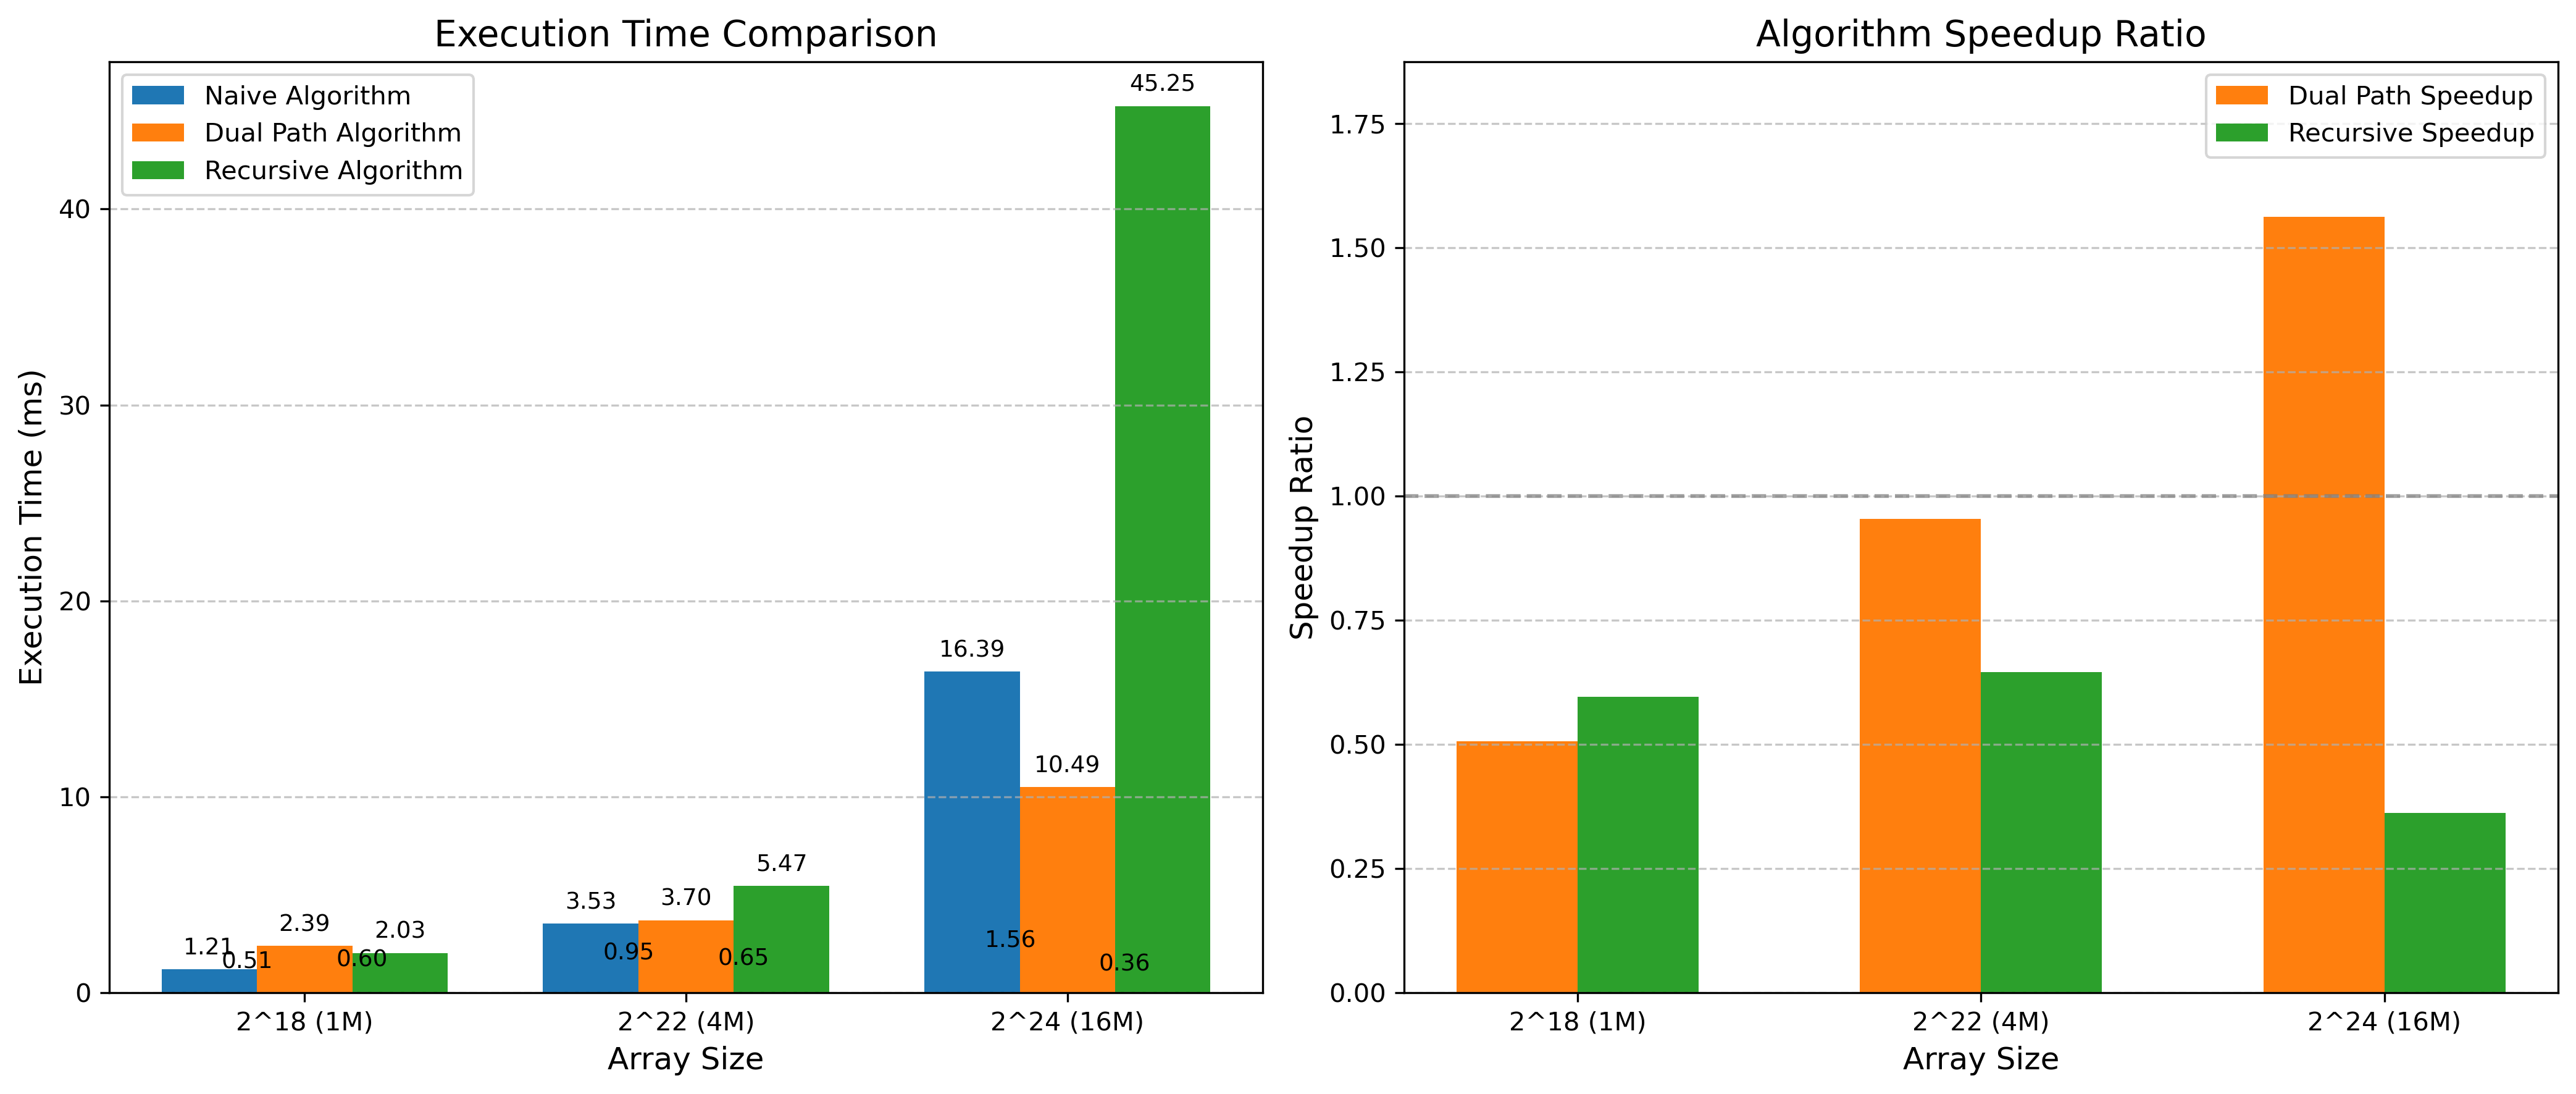
\includegraphics[width=\textwidth]{sum_array_performance.png}
    \caption{数组求和性能比较}
    \label{fig:sum_array_performance}
  \end{subfigure}
  \hfill
  \begin{subfigure}[b]{0.45\textwidth}
    \centering
    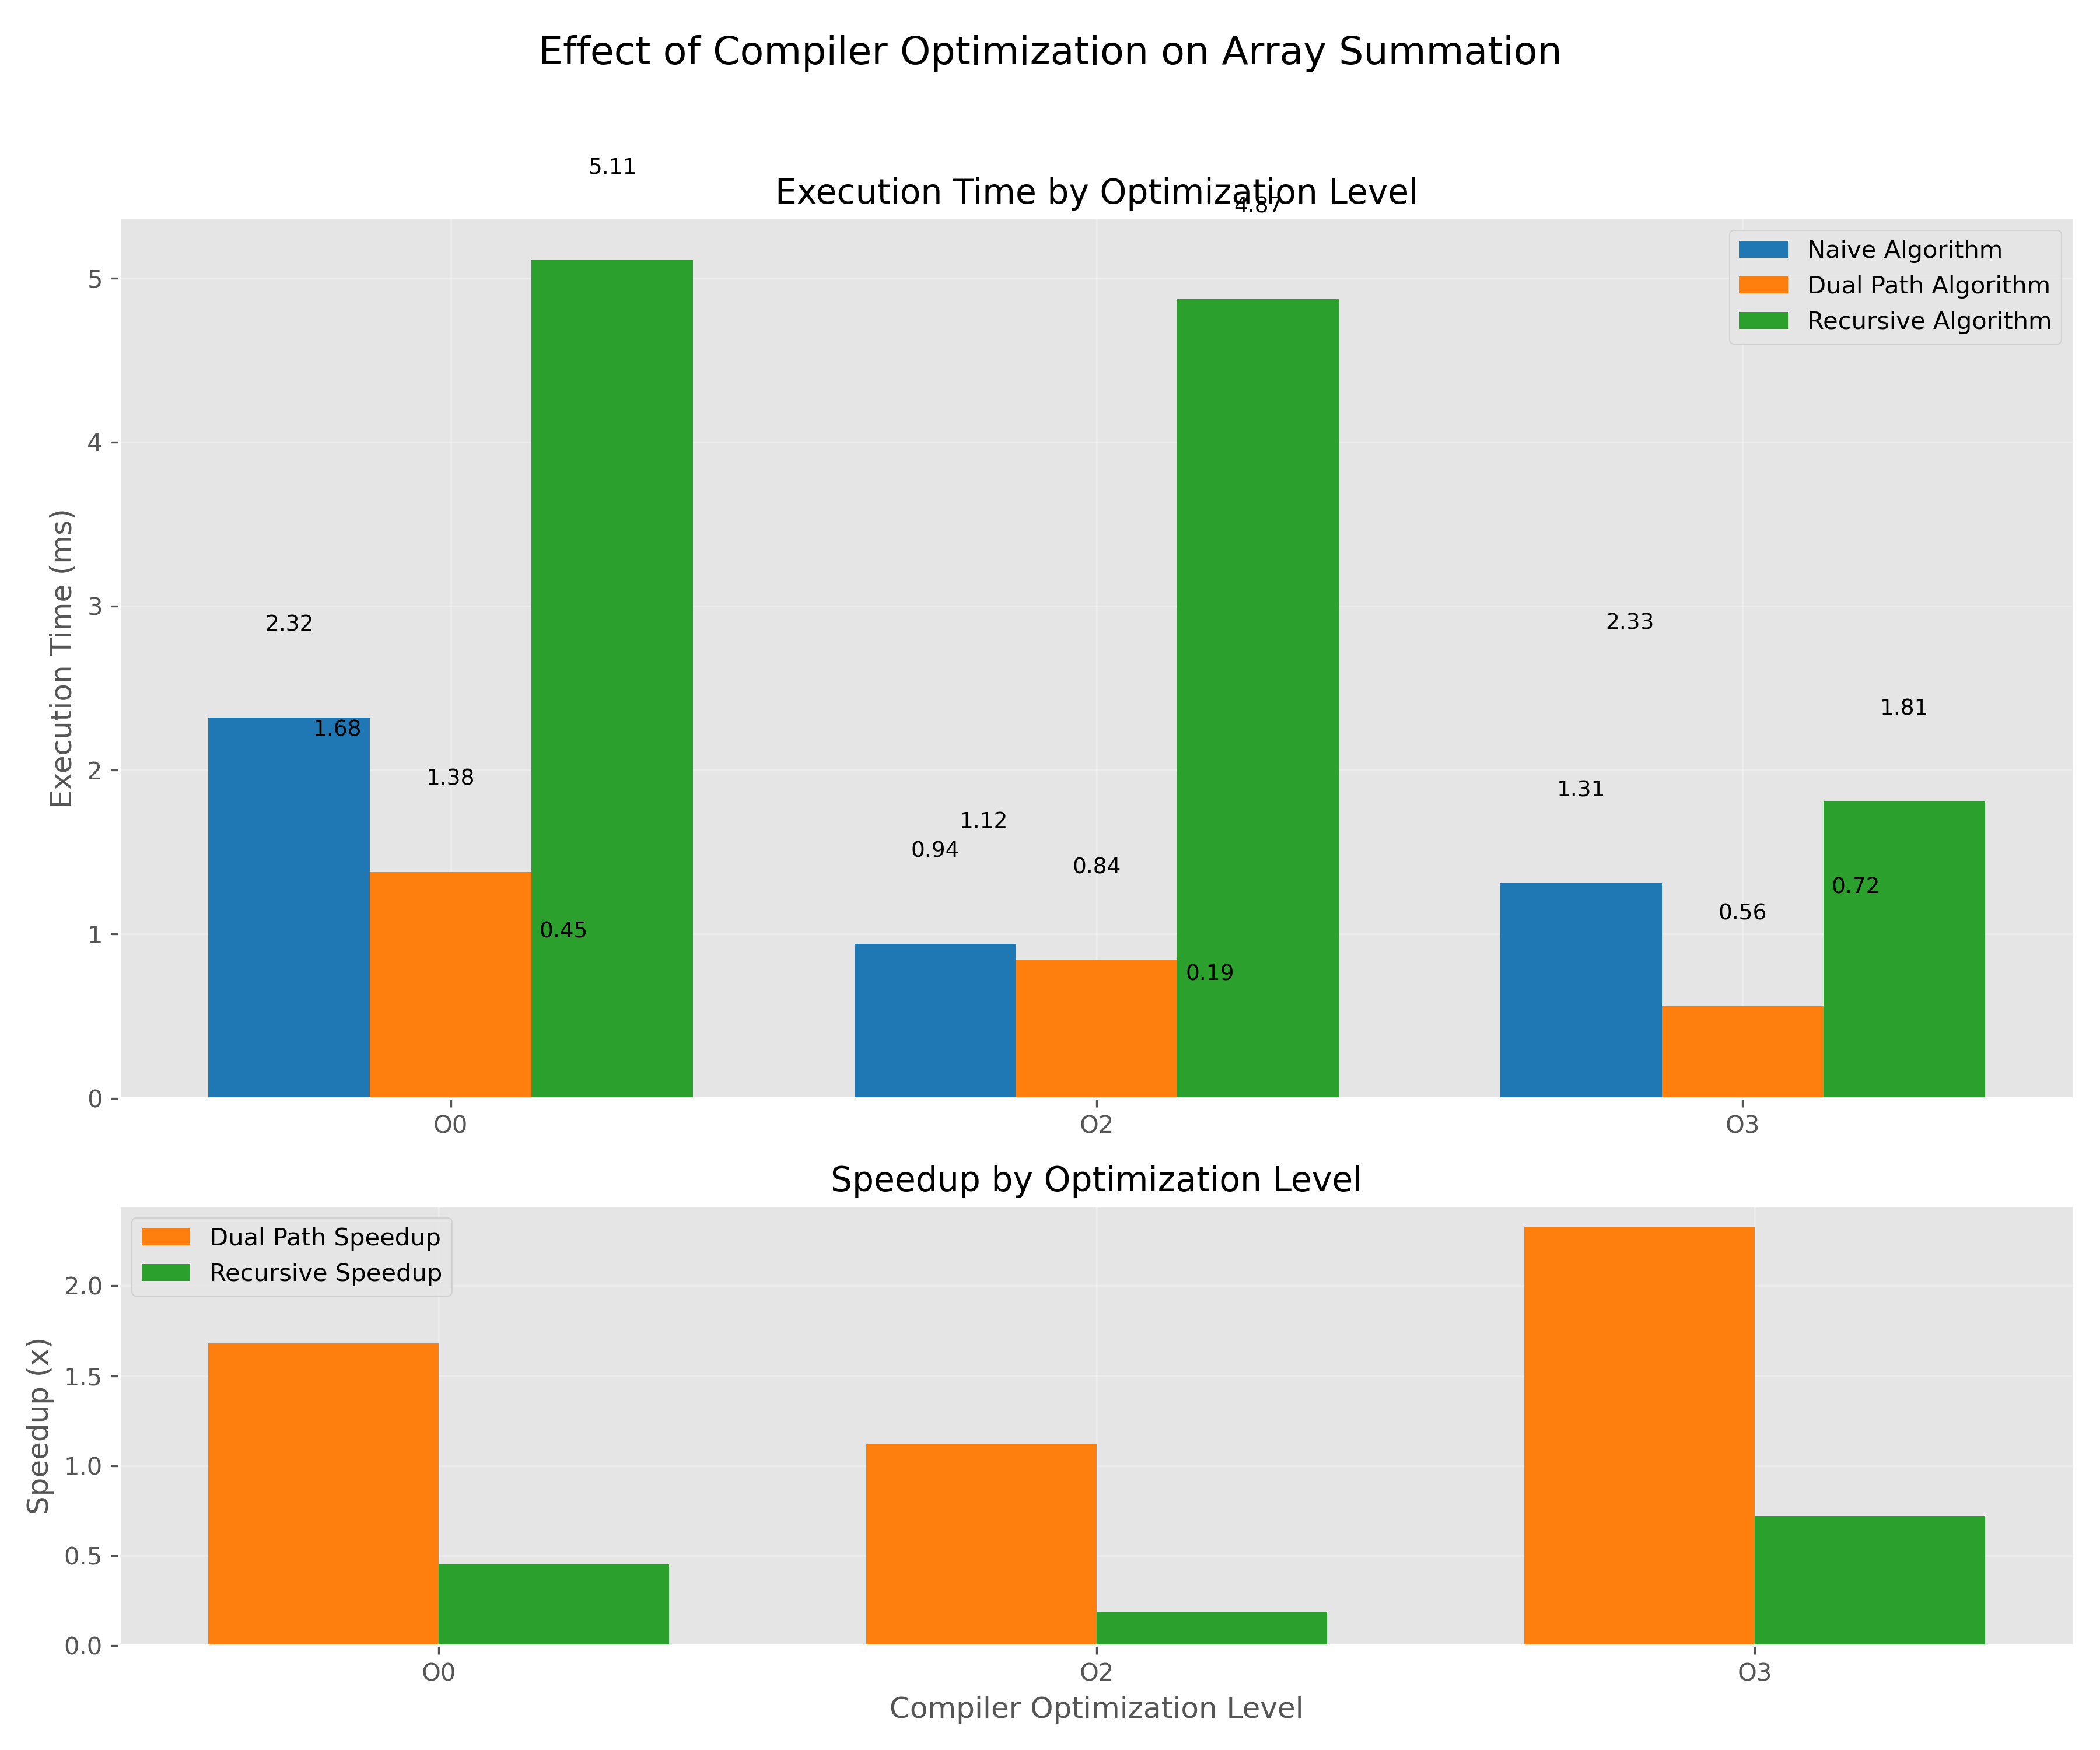
\includegraphics[width=\textwidth]{compiler_opt_sum.png}
    \caption{编译器优化对数组求和的影响}
    \label{fig:compiler_opt_sum}
  \end{subfigure}
  \caption{数组求和实验结果}
  \label{fig:array_results}
\end{figure}

\textbf{图9 数组求和算法对比}:左图展示了不同算法随数据规模增长的性能变化。朴素算法(蓝色)在较小数据规模(2\textsuperscript{18}、2\textsuperscript{22})下表现最佳;双链路算法(橙色)仅在较大数据规模(2\textsuperscript{24})上有效,获得1.56倍加速;递归算法(绿色)性能整体较差,在所有测试规模上都慢于朴素算法。从右图加速比可以看出,随着数据规模增大,双链路算法的加速比逐渐提高,而递归算法则始终表现不佳。这说明优化方法的有效性与数据规模密切相关,并不是所有优化都能在所有场景下获益。

\textbf{图10 编译器优化影响}:上图展示了优化级别对算法性能的影响。双链路算法在O3级别下表现最佳;递归算法O3级别下得到显著改善。下图显示O3级别下双链路算法获得了更高的加速比。这表明编译器优化能够识别并强化某些算法中的并行性潜力,特别是对指令级并行度较高的代码。

\subsection{profiling}

\subsubsection{平凡算法}

平凡算法的cachegrind分析显示缓存未命中率很低(约0.1\%),因为数组顺序访问具有良好的空间局部性,主要瓶颈是指令间的数据依赖。

\subsubsection{超标量优化算法}

双链路算法的缓存未命中率与平凡算法相当,性能提升主要来自于减少了数据依赖,允许CPU更好地进行流水线操作,两个独立的累加操作可以并行执行,提高了CPU利用率。

\subsection{架构对比分析}

双链路算法在两种架构上都有效,但加速效果与数据规模关系显示不同模式。这表明指令级并行优化在不同架构上的有效性相对稳定,不像缓存优化那样受硬件差异影响显著。如图\ref{fig:arch_comparison}(b)所示。

\section{实验总结和思考}

\subsection{对比2个实验的异同}

两个实验在优化效果、瓶颈和优化侧重点上表现出明显差异:
\begin{itemize}
  \item \textbf{优化效果}:矩阵-向量乘法获得7.2倍加速,数组求和仅1.56倍加速
  \item \textbf{瓶颈差异}:矩阵乘法主要受缓存未命中影响,数组求和受指令级数据依赖限制
  \item \textbf{优化侧重}:矩阵乘法优化内存访问模式,数组求和优化指令级并行
\end{itemize}

\subsection{总结}

本实验得出以下核心结论:
\begin{enumerate}
  \item 缓存优化对性能提升的贡献通常大于指令级并行优化,特别是对于大数据集
  \item 不同硬件架构对优化策略的响应有显著差异,x86对缓存优化更敏感,ARM在ILP优化方面表现出色
  \item 算法设计应首先考虑内存访问模式,然后才是并行性和其他微优化
  \item 编译器优化能大幅提升代码性能,但不能完全弥补算法本身的缺陷
\end{enumerate}

这些发现对高性能计算、嵌入式系统和跨平台软件开发都有重要指导意义。未来工作可探索SIMD向量化、多线程并行等更高级优化策略。

\clearpage
% 参考文献章节样式定义
\def\bibsection{
  \section*{\refname\markboth{\refname}{\refname}}%
  \addcontentsline{toc}{section}{\refname}%
  \begingroup
    \fontsize{12}{14}\selectfont% 章节标题字体大小
    \vspace{0.8em}
  \endgroup
}

% 确保所有参考文献都被包含
\nocite{*}

% 使用纯natbib方式处理参考文献
\bibliography{reference.bib}

\end{document} 